\documentclass[conference]{IEEEtran}
\IEEEoverridecommandlockouts
% The preceding line is only needed to identify funding in the first footnote. If that is unneeded, please comment it out.
%Template version as of 6/27/2024

\usepackage{cite}
\usepackage{amsmath,amssymb,amsfonts}
\usepackage{algorithmic}
\usepackage{graphicx}
\usepackage{textcomp}
\usepackage{xcolor}
\usepackage{subcaption}
\usepackage{booktabs}
\usepackage{url}
\usepackage{microtype}
\usepackage{listings}
\usepackage{float}
\usepackage{multirow}

\def\BibTeX{{\rm B\kern-.05em{\sc i\kern-.025em b}\kern-.08em
		T\kern-.1667em\lower.7ex\hbox{E}\kern-.125emX}}

% Listings configuration
\lstset{
	basicstyle=\ttfamily\footnotesize,
	breaklines=true,
	breakatwhitespace=true,
	frame=single,
	columns=fullflexible,
	keepspaces=true
}

\begin{document}
	
	\title{The EC2 Sweet Spot: A Cost-Efficiency Analysis of Video Codecs on AWS C, M, and T-Family Instances\\
	\thanks{This study was financed in part by the Coordenação de Aperfeiçoamento de Pessoal de Nível Superior (CAPES)}
}
	
	\author{\IEEEauthorblockN{1\textsuperscript{st} Breno Vasconcelos}
		\IEEEauthorblockA{\textit{Centro de Informática} \\
			\textit{Universidade Federal de Pernambuco (UFPE)}\\
			Recife, Pernambuco, Brazil \\
			bjrv@cin.ufpe.br \\
			ORCID: 0009-0005-6451-8313}
		\and
		\IEEEauthorblockN{2\textsuperscript{nd} Carlos Ferraz}
		\IEEEauthorblockA{\textit{Centro de Informática} \\
			\textit{Universidade Federal de Pernambuco (UFPE)}\\
			Recife, Pernambuco, Brazil \\
			cagf@cin.ufpe.br \\
			ORCID: 0000-0002-4861-0719}
	}
	
	\maketitle
	
	\begin{abstract}
		The diverse landscape of cloud instance types presents significant resource allocation challenges for video compression. This study investigates cost optimization strategies across Burstable (T), General Purpose (M), and Compute Optimized (C) instance families for Video-as-a-Service (VaaS) workloads. Initial benchmarking reveals that while Compute instances deliver the fastest raw performance, smaller Burstable instances are up to 29× more cost-efficient when comparing opposite performance extremes (e.g., \texttt{t3.micro} vs \texttt{c5.4xlarge}). However, leveraging this efficiency for large divisible workloads introduces severe provisioning bottlenecks. Our analysis quantifies this operational overhead at approximately 70\% of total processing time. By utilizing custom Amazon Machine Images (AMIs), we successfully eliminated this bottleneck. This optimization unlocked horizontal scaling as a universally superior strategy. Across all three families, clusters of ten optimized \texttt{micro/large} instances consistently outperformed the processing speed of the largest available vertical instances (\texttt{2xlarge/4xlarge}) while maintaining competitive or vastly superior economics. For the T-family, the cluster achieved a 1.28× speedup alongside a 75.5\% cost reduction. This study demonstrates that quantifying and eliminating cloud provisioning overhead is the critical prerequisite for high-performance, cost-efficient VaaS resource allocation.
	\end{abstract}
	
	\begin{IEEEkeywords}
		Cloud Management, Cost Optimization Strategies, Resource Allocation, VaaS, Video Codecs, Parallel Encoding
	\end{IEEEkeywords}
	
	\section{Introduction}
	
	Cloud-based video processing has become fundamental to modern media delivery, driving the expansion of Video-as-a-Service (VaaS) platforms for streaming, surveillance, and large-scale content distribution. However, achieving cost-effective performance in cloud environments presents significant cloud management challenges, as diverse instance types create complex trade-offs between computational capacity, resource allocation, and operational expenses \cite{b1,b17}.
	
	While prior research has established foundations in cloud resource optimization and video encoding performance, specific cost optimization strategies targeting burstable compute instances remain underexplored. Previous studies have either focused on general cloud benchmarking without video encoding specialization \cite{b1}, examined encoding performance without comprehensive cost analysis \cite{b3}, or addressed multi-cloud scheduling without considering the unique characteristics of media processing workloads \cite{b20}. This gap is particularly relevant for burstable instances, which offer temporary high performance at low baseline cost but introduce operational complexities for divisible workloads like video compression.
	
	While emerging standards like Versatile Video Coding (VVC) offer superior compression, their extreme computational demands currently make them unsuitable for cost-effective deployment on minimal burstable instances. Therefore, this study focuses on established codecs (H.264, H.265, and VP9) that represent the vast majority of current commercial media pipelines.
	
	This study addresses these limitations through a comprehensive analysis of AWS T (Burstable), M (General Purpose), and C (Compute Optimized) family instances for video encoding workloads. Our research aims to answer three key questions: (1) How do cost-performance profiles compare across different instance families? (2) What operational overheads affect parallel encoding efficiency in horizontally scaled architectures? (3) Can provisioning optimizations eliminate these overhead bottlenecks sufficiently to make small-instance clusters more effective than vertical scaling?
	
	Our primary contribution to cloud management is the quantification and elimination of cloud provisioning overhead for episodic workloads. We demonstrate that in unoptimized parallel architectures, operational provisioning accounts for roughly 70\% of total processing time. By developing a custom Amazon Machine Image (AMI) framework, we successfully eliminated this bottleneck. This foundational optimization fundamentally shifted the scaling economics: it enabled optimized horizontal clusters of small instances to consistently outperform the processing speed of the largest vertical instances across all tested families (e.g., 1.28× speedup for T-family, 1.22× for M-family, and 1.17× for C-family).
	
	These findings have practical implications for organizations deploying VaaS platforms. By proving that provisioning overhead can be systematically erased, we establish that properly configured horizontal scaling is not merely a cost-saving alternative, but a superior, performance-maximizing approach for divisible cloud workloads.
	
	This paper is structured as follows: Section~\ref{rel_works} reviews related work in cloud resource optimization and video processing. Section~\ref{met} details our experimental methodology across three phases. Section~\ref{experiments} presents corresponding results. Section~\ref{limitations} discusses findings and threats to validity, and Section~\ref{conclusion} summarizes contributions and outlines future research directions.
	
	\section{Related Works}
	\label{rel_works}
	
	Video processing computational resource optimization presents research challenges due to modern codec complexity. Advanced standards like Versatile Video Coding (VVC) introduce sophisticated tools that increase computational demands, driving research into algorithmic optimizations \cite{b15, b16}. While prior work, such as that by \textbf{Dancheva et al.} \cite{b3}, focuses on comparative encoding performance, our investigation shifts the focus to the cloud infrastructure itself, analyzing its performance and cost-effectiveness for practical deployment.
	
	Cloud resource optimization has been studied from multiple perspectives. Prior work includes cost-driven provisioning methodologies for scientific computing, as demonstrated by \textbf{Álvarez et al.} \cite{b2}, and surveys categorizing resource management strategies \cite{b4}. Our research extends this foundation by demonstrating that properly optimized horizontal architectures can simultaneously outperform vertical scaling for video encoding workloads in both processing speed and cost-efficiency.
	
	Recent work by \textbf{Jiang et al.} \cite{b20} introduces PIVOT, a cloud-agnostic framework that addresses cost-aware scheduling in multi-cloud environments. Their approach tackles significant challenges in cross-cloud data analysis, including infrastructure heterogeneity and prohibitive egress costs. While PIVOT focuses on multi-cloud workflow orchestration for big data applications, our work complements this by providing a granular analysis of cost-performance trade-offs within a single cloud provider's burstable instance family, specifically for video encoding workloads.
	
	Recent research extensively explores the nuances of video encoding deployments on cloud infrastructure. \textbf{Moina-Rivera et al.} \cite{b22} provided a comprehensive systematic review of cloud and edge media encoding and transcoding techniques, highlighting the critical architectural challenges and emphasizing the economic benefits of adaptive, pay-as-you-go cloud models. While their review effectively charts the technological landscape, our study complements this by contributing an empirical case study targeting burstable instance cost optimization.
	
	\textbf{Zabrovskiy et al.} \cite{b21} introduced FSpot, an intelligent scheduling heuristic explicitly targeting Amazon EC2 spot instances to minimize video encoding costs. Their approach reduces expenses by rapidly benchmarking and dynamically estimating encoding speeds for cheap but volatile computing units. Similarly, \textbf{Silva} \cite{b19} analyzed spot instance pricing strategies to minimize multi-cloud execution costs. While these respective strategies provide extreme economic incentives by leveraging unpredictable spot markets (typically 70-90\% cheaper than On-Demand), they introduce intrinsic preemption risks that may force workload restarts. Our methodology establishes a deterministic alternative: carefully orchestrated horizontal scaling on stable burstable instances can comparably achieve outstanding cost-efficiency while circumventing the risks of sudden instance termination, guaranteeing completion without interruption.
	
	The multi-objective nature of cloud optimization problems has been well-established. Studies such as \textbf{Katsenou et al.} \cite{b8} provide thorough analyses of energy efficiency trade-offs across different codecs and hardware platforms. Furthermore, investigations into workload-specific instance selection \cite{b14}, such as those by \textbf{Maas et al.} \cite{b1}, comprehensively evaluated the cost-performance trade-offs for parallel applications across 104 HPC and general-purpose instances, revealing that tailoring instance selection to specific cloud resources yields significant improvements. Our work aligns with this approach but introduces a specialized focus on video encoding.

	In a related line of inquiry, \textbf{Maas et al.} \cite{b23} specifically examined how thread scalability characteristics influence performance and cost optimization for parallel workloads across three major cloud providers. They demonstrated that matching an application's thread-level parallelism to the appropriate instance type prevents unnecessary expenditures on redundant cores. While their analysis focuses heavily on general HPC applications, our research applies analogous scalability principles directly to divisible video encoding workloads on burstable instances to deliberately mitigate operational overhead.
	
	Benchmarking methodologies represent a critical dimension of cloud performance research. Broad comparative studies illustrate the heterogeneity in cloud technologies, highlighting challenges in establishing direct performance comparisons \cite{b18, b1}. Our methodology addresses this challenge through environmental standardization, using containerized execution environments that align with the reproducible frameworks advocated by studies such as \textbf{Ferreira et al.} \cite{b9}.
	
	Our research addresses cloud performance variability through empirical measurement. We quantify variability across 30 trials per configuration, establishing baseline performance profiles for cost-efficiency analysis. This data-driven approach complements predictive modeling techniques proposed in prior work \cite{b10, b11}.
	
	The architectural principles underlying our parallel processing case study draw from established distributed systems concepts. The fundamental strategy of decomposing large, divisible workloads to optimize cost efficiency has been demonstrated in contexts such as task scheduling in fog-cloud environments \cite{b12, b13}. Our contribution lies in applying these principles to a specialized yet practically significant domain: parallel video encoding within public cloud infrastructure, with particular emphasis on quantifying and mitigating provisioning overhead.
	
	Table~\ref{tab:comparative_analysis} provides a comparison of related research, illustrating how our work complements and extends existing literature. While previous studies have established valuable foundations in their respective domains, our research provides an integrated analysis specifically addressing cost-efficiency trade-offs in burstable instances and parallel video encoding architectures, with particular emphasis on operational overhead quantification and practical optimization strategies that bridge identified research gaps.
	
	\begin{table*}[!htbp]
		\centering
		\caption{Comparison of related works in cloud resource optimization and video processing}
		\label{tab:comparative_analysis}
		\begin{tabular}{|p{0.15\linewidth}|p{0.18\linewidth}|p{0.28\linewidth}|p{0.28\linewidth}|}
			\hline
			\textbf{Study} & \textbf{Focus} & \textbf{Contributions} & \textbf{Gaps Addressed} \\
			\hline
			Álvarez et al. \cite{b2} & Scientific workloads & Cost-aware provisioning & No media processing focus \\
			\hline
			Dancheva et al. \cite{b3} & Video encoding performance & Encoding time comparison & Limited cost analysis \\
			\hline
			Jiang et al. \cite{b20} & Multi-cloud scheduling & Cost-aware framework for cross-cloud workflows & Big data focus, limited video processing analysis \\
			\hline
			Maas et al. \cite{b1} & Broad cloud benchmarking & Instance performance analysis & No video encoding specialization \\
			\hline
			Ferreira et al. \cite{b9} & Benchmarking methodologies & Reproducible frameworks & No video encoding application \\
			\hline
			Katsenou et al. \cite{b8} & Energy efficiency & Codec energy analysis & Embedded devices focus \\
			\hline
            Moina-Rivera et al. \cite{b22} & Cloud/Edge video encoding & Systematic literature review of media encoding architecture & Review only, lacks novel burstable empirical case studies \\
            \hline
            Zabrovskiy et al. \cite{b21} & Spot instance cost optimization & FSpot scheduling heuristic for minimal cost video encoding & Relies on volatile spot instances; risk of interruption \\
            \hline
            Maas et al. \cite{b23} & Thread scalability & Workload-specific thread scalability evaluation across clouds & Focused on generic HPC, lacks video encoding specialization \\
			\hline
			Our Work & \textbf{Burstable instances for video encoding} & Size-efficiency trade-offs; Overhead quantification; AMI optimization; Scaling comparison & Burstable instance focus; Parallel overhead measurement; Divisible workload optimization; Practical AMI strategies \\
			\hline
		\end{tabular}
	\end{table*}
	
	\section{Experimental Methodology}
	\label{met}
	
	This study employed an experimental methodology to investigate the relationship between computational cost and performance for video encoding in cloud environments. The research was conducted on AWS infrastructure in the us-east-1 region and comprised three sequential phases.
	
	\subsection{Phase 1: Validation of Processor Homogeneity}
	\label{met:validation-processor-homogeneity}
	
	To address hardware heterogeneity in cloud environments, we implemented a verification protocol for hardware consistency. We deployed 100 instances of each configuration type (T, M, and C families) across all availability zones (a-f) within us-east-1, all initialized with Ubuntu 22.04 LTS.
	
	Each instance executed \texttt{cat /proc/cpuinfo} to extract processor specifications. Analysis confirmed hardware variation across availability zones, consistent with prior cloud studies \cite{b2, b5, b6, b7}. For the T-family (\texttt{t3.micro}) in zone 'a', 98 instances featured the Xeon 8259CL while 2 instances featured the older Xeon 8175M. Similar heterogeneity surfaced in other families: the M-family (\texttt{m5.large}) in zone 'c' split 60/40 between 8259CL and 8175M processors, and the C-family (\texttt{c5.large}) in zone 'b' split 74/26 between 8275CL and 8124M variants (Table \ref{tab:processors}).
	
	\begin{table}[H]
		\centering
		\caption{Processor distribution across availability zones (100 instances per family)}
		\label{tab:processors}
		\begin{tabular}{|c|c|c|c|}
			\hline
			\textbf{Family} & \textbf{Avail. Zone} & \textbf{Processor Architecture} & \textbf{Count} \\ \hline
			\multirow{2}{*}{T (\texttt{t3.micro})} & a & Xeon(R) 8259CL @ 2.50GHz & 98 \\ \cline{2-4}
			& a & Xeon(R) 8175M @ 2.50GHz & 2 \\ \hline
			\multirow{2}{*}{M (\texttt{m5.large})} & c & Xeon(R) 8259CL @ 2.50GHz & 60 \\ \cline{2-4}
			& c & Xeon(R) 8175M @ 2.50GHz & 40 \\ \hline
			\multirow{2}{*}{C (\texttt{c5.large})} & b & Xeon(R) Platinum 8275CL @ 3.00GHz & 74 \\ \cline{2-4}
			& b & Xeon(R) Platinum 8124M @ 3.00GHz & 26 \\ \hline
		\end{tabular}
	\end{table}
	
	To eliminate hardware heterogeneity as a confounding variable, we standardized our benchmarks by exclusively selecting instances with the dominant CPU architecture for each specific instance type (e.g., Xeon 8259CL for T and M families, Xeon 8275CL for C family). During provisioning, instances underwent rapid architectural validation, with any non-conforming instances immediately terminated and automatically replaced before executing the video compression workloads.
	
	\subsection{Phase 2: Initial Performance Benchmarks}
	\label{execution-initial-performance-benchmarks}
	
	We established experimental instances for video compression evaluation. We used a Docker container environment pre-configured with FFmpeg and codec support for H.264/AVC, H.265/HEVC, and VP9.
	
	The experimental workload utilized 1080p standard test sequences representing typical Video-on-Demand (VOD) content with mixed motion. We deliberately selected 30-second video segments to minimize the relative impact of process initialization overhead (container startup, FFmpeg loading) on the execution time, which can otherwise mask true CPU performance differences in shorter chunks. Each condition was replicated 30 times. Video compression was evaluated using this FFmpeg command:
	
	\begin{center}
		{\ttfamily\scriptsize
			\fbox{
				\begin{minipage}{0.9\linewidth}
					ffmpeg -i input.mp4 -c:v <codec> -preset slow -b:v 2M \\
					\hspace{15pt}-threads <n> output.mp4
				\end{minipage}
			}
		}
	\end{center}
	
	The \texttt{<codec>} parameter evaluated \texttt{libx264}, \texttt{libx265}, and \texttt{libvpx-vp9}. The \texttt{<n>} parameter was tested with 1, 3, 5, and 10 threads. Encoding duration was recorded and cost calculated based on instance pricing.
	
	\subsection{Phase 3: Horizontal vs. Vertical Scaling Analysis}
	
	We conducted a case study comparing horizontal versus vertical scaling for a 10-minute video workload. This duration represents standard user-generated content (e.g., typical YouTube uploads)—large enough to require segmentation for optimal processing, yet small enough to benchmark rapid batch processing. The scaling analysis compared three architectural strategies: horizontal scaling using ten t3.micro instances each processing one-minute segments; vertical scaling with a single t3.2xlarge instance processing the complete video; and a baseline configuration with one t3.micro instance processing the video sequentially.
	
	The investigation comprised two phases: Dynamic Provisioning, with instances launched from a base Ubuntu image; and Optimized Provisioning, with instances launched from a custom machine image. Both phases measured processing duration and computational costs.
	
	Beyond parallelization, this architectural division provides a critical operational advantage in fault tolerance. In the horizontal configuration, if a single \texttt{t3.micro} node fails during processing, only its specific 1-minute segment requires re-processing (approximately 6 seconds of recovery computation). Conversely, a failure in the vertical \texttt{t3.2xlarge} instance near completion requires re-processing the entire 10-minute video (over 90 seconds of lost computation)—representing a 15× improvement in failure recovery granularity.
	
	Execution time metrics were recorded with millisecond resolution. For Phase 2 benchmarks, each configuration command was repeated 30 times. We computed descriptive statistics across these repetitions, calculating 95\% Confidence Intervals (Student's t-distribution) for all configurations to confirm behavioral stability. For Phase 3, due to the extended duration and cloud provisioning logistics of the 10-minute parallel workloads, each cross-family macro-architecture configuration was repeated $n=10$ times. To account for this reduced sample size while maintaining analytical rigor, we applied a derived, conservative $\pm$3\% error margin to Phase 3 results. This margin represents the maximum empirical relative error observed across the exhaustive $n=30$ Phase 2 benchmarks, safely establishing an upper-bound confidence interval for the scaling behaviors. Statistical analysis further included Shapiro-Wilk tests, Levene's tests, and Welch's t-tests.
	
	
	\section{Experimental Results and Analysis}
	\label{experiments}
	
	This section presents results from our three-phase experimental investigation, corresponding to the methodological phases in Section 3.
	
	\subsection{Phase 1 Results: Processor Homogeneity Validation}
	\label{results-phase1}
	
	Our validation of computational homogeneity across AWS availability zones revealed hardware heterogeneity, consistent with prior cloud computing research. As detailed in Table~\ref{tab:processors}, we observed variation in processor architectures within the same instance type and availability zone.
	
	For minimal instance configurations (T-family) investigated in availability zone \texttt{a}, 98\% of instances used Intel Xeon Platinum 8259CL processors, while 2\% used 8175M processors. M-family instances exhibited an even more pronounced split (60\%/40\%), reinforcing the severity of the hardware lottery. This finding required our experimental control strategy to ensure valid performance comparisons. By standardizing on the dominant processor architecture for each instance type, we successfully eliminated hardware heterogeneity as a confounding variable across all subsequent phases.
	
	Preliminary measurements showed uncontrolled hardware variation caused up to 15\% performance deviations, establishing the need for controlled benchmarking.
	
	
	
	
	
	
	
	
	
	
	
	
	\subsection{Phase 2 Results: Initial Performance Benchmarks}
	\label{results-phase2}
	
	This study evaluated video compression performance across H.264, H.265, and VP9 codecs on AWS EC2 instances with varying thread configurations. Performance was assessed through Compression Time (seconds), Efficiency (Equation~\ref{eq:efficiency}), and Total Cost per operation.
	
	\subsubsection{Efficiency and Cost Calculation}
	\label{efficiency-calculation}
	
	Two complementary metrics were employed: Efficiency (Equation~\ref{eq:efficiency}) for comparative performance-cost analysis and Total Cost (Equation~\ref{eq:total_cost}) for direct monetary assessment.
	
	\begin{equation}
		\text{Efficiency} = \frac{1}{(\text{cost}/3600) \times \text{time}}
		\label{eq:efficiency}
	\end{equation}
	
	\begin{equation}
		\text{Total Cost} = (\text{hourly cost}/3600) \times \text{time}
		\label{eq:total_cost}
	\end{equation}
	
	The cost variable corresponds to hourly instance rates from Table~\ref{tab:experimental_configurations}, while time represents compression duration in seconds. Mathematically, our Efficiency definition functions as an \textit{Inverse Cost-Delay Product}, analogous to the Energy-Delay Product used in hardware architecture. By taking the reciprocal of the product of time and cost (which is effectively time $\times$ cost-per-time $\times$ time, or $cost \times time^2$), this non-linear metric explicitly and heavily penalizes configurations that are either excessively slow or disproportionately expensive. Unlike raw ``speedup'' (which ignores budget) or ``work per dollar'' (which ignores latency), the Inverse Cost-Delay Product answers the multi-objective optimization requirements of cloud management by rewarding the true ``sweet spot'': configurations that simultaneously minimize infrastructure expenditure and execution delay. Total Cost (Equation~\ref{eq:total_cost}) complements this by providing the actual monetary cost per operation.
	
	\begin{table}[H]
		\centering
		\caption{Experimental instance configurations}
		\label{tab:experimental_configurations}
		\begin{tabular}{|l|c|c|c|c|}
			\hline
			\textbf{Instance Type} & \textbf{vCPU} & \textbf{RAM (GiB)} & \textbf{Cost/hour (USD)}  \\
			\hline
			t2.micro & 1 & 1 & 0.0116  \\
			t3.micro & 2 & 1 & 0.0104 \\
			t3.small & 2 & 2 & 0.0208 \\
			t3.medium & 2 & 4 & 0.0416 \\
			t3.large & 2 & 8 & 0.0832 \\
			t3.xlarge & 4 & 16 & 0.1664 \\
			t3.2xlarge & 8 & 32 & 0.3328 \\
			\hline
			m5.large & 2 & 8 & 0.0960 \\
			m5.xlarge & 4 & 16 & 0.1920 \\
			m5.2xlarge & 8 & 32 & 0.3840 \\
			m5.4xlarge & 16 & 64 & 0.7680 \\
			\hline
			c5.large & 2 & 4 & 0.0850 \\
			c5.xlarge & 4 & 8 & 0.1700 \\
			c5.2xlarge & 8 & 16 & 0.3400 \\
			c5.4xlarge & 16 & 32 & 0.6800 \\
			\hline
		\end{tabular}
	\end{table}
	
	\subsubsection{Performance Analysis}
	
	Table \ref{tab:final_comparison_consistent} presents descriptive statistics for Compression Time, Efficiency, and Total Cost across all experimental configurations. The analysis reveals performance patterns extending beyond the expected correlation between instance capability and processing speed.
	
	\begin{table*}[h]
		\centering
		\caption{Descriptive statistics for compression time (seconds), efficiency, and total cost across all experimental configurations}
		\label{tab:final_comparison_consistent}
		\resizebox{\textwidth}{!}{
			\begin{tabular}{ll|rrrrr|rrrrr|rrrrr}
				\toprule
				& & \multicolumn{5}{c|}{H.264} & \multicolumn{5}{c|}{H.265 (libx265)} & \multicolumn{5}{c}{VP9 (libvpx-vp9)} \\
				\cmidrule(lr){3-7} \cmidrule(lr){8-12} \cmidrule(lr){13-17}
				& & \multicolumn{4}{c}{Compression Time (s)} & \multicolumn{1}{c|}{Eff. | Cost (\$)} & \multicolumn{4}{c}{Time (s)} & \multicolumn{1}{c|}{Eff. | Cost (\$)} & \multicolumn{4}{c}{Time (s)} & \multicolumn{1}{c}{Eff. | Cost (\$)} \\
				Instance Type & Threads & Median & Std & Min & Max & (Median) & Median & Std & Min & Max & (Median) & Median & Std & Min & Max & (Median) \\
				\midrule
				t2.micro & 1 thread & \textbf{2.6350} & 0.0125 & 2.6125 & 2.6625 & \textbf{117,678} | 0.0000085 & 5.0727 & 0.0259 & 5.0227 & 5.1136 & 61,185 | 0.0000163 & 15.1205 & 0.0559 & 15.0461 & 15.2922 & 20,551 | 0.0000486 \\
				t2.micro & 3 thread & 2.7766 & 0.0211 & 2.7433 & 2.8485 & 111,949 | 0.0000089 & 5.0227 & 0.0293 & 4.9592 & 5.1073 & 61,863 | 0.0000162 & \textbf{14.7580} & 0.0470 & 14.7042 & 14.9585 & \textbf{21,059} | 0.0000475 \\
				t2.micro & 5 thread & 2.7061 & 0.0109 & 2.6892 & 2.7321 & 114,752 | 0.0000087 & 4.8909 & 0.0239 & 4.8423 & 4.9416 & 63,534 | 0.0000157 & 15.4243 & 0.0900 & 15.3474 & 15.7989 & 20,155 | 0.0000496 \\
				t2.micro & 10 thread & 2.7638 & 0.0155 & 2.7383 & 2.8035 & 112,389 | 0.0000089 & \textbf{4.8818} & 0.0260 & 4.8389 & 4.9319 & \textbf{63,666} | 0.0000157 & 14.8821 & 0.0443 & 14.8242 & 15.0429 & 20,880 | 0.0000479 \\
				\midrule
				t3.micro & 1 thread & 2.8227 & 0.0280 & 2.8019 & 2.9554 & 122,912 | 0.0000081 & 4.5000 & 0.1850 & 4.4746 & 5.4597 & 77,294 | 0.0000130 & 17.5833 & 0.2616 & 17.4581 & 18.5267 & 19,836 | 0.0000508 \\
				t3.micro & 3 thread & 2.5310 & 0.0541 & 2.5235 & 2.8314 & 137,337 | 0.0000073 & 4.3478 & 0.0621 & 4.3179 & 4.6603 & 79,985 | 0.0000125 & 17.7470 & 0.3460 & 17.5258 & 18.8740 & 19,655 | 0.0000513 \\
				t3.micro & 5 thread & \textbf{2.5307} & 0.0677 & 2.2560 & 2.7556 & \textbf{137,352} | 0.0000073 & 4.3159 & 0.0299 & 4.2833 & 4.3765 & 80,471 | 0.0000125 & 17.5244 & 0.2950 & 17.3751 & 18.7260 & 19,897 | 0.0000507 \\
				t3.micro & 10 thread & 2.5702 & 0.0196 & 2.4820 & 2.6076 & 135,274 | 0.0000074 & \textbf{4.2952} & 0.1018 & 3.7388 & 4.3470 & \textbf{80,955} | 0.0000124 & \textbf{17.5015} & 0.1475 & 17.3627 & 17.9877 & \textbf{19,929} | 0.0000506 \\
				\midrule
				t3.small & 1 thread & 2.8409 & 0.1740 & 2.8277 & 3.8000 & 61,870 | 0.0000164 & 4.4990 & 0.1693 & 4.4650 & 5.3317 & 38,845 | 0.0000260 & \textbf{17.7128} & 0.2013 & 17.5151 & 18.1245 & \textbf{9,842} | 0.0001023 \\
				t3.small & 3 thread & 2.5482 & 0.2160 & 2.5307 & 3.7303 & 68,969 | 0.0000147 & 4.3636 & 0.1248 & 4.1519 & 4.8299 & 40,050 | 0.0000252 & 17.8011 & 0.2749 & 17.5453 & 18.5326 & 9,793 | 0.0001030 \\
				t3.small & 5 thread & \textbf{2.5303} & 0.0679 & 2.5216 & 2.8993 & \textbf{69,466} | 0.0000146 & 4.3218 & 0.1488 & 4.2909 & 4.9702 & 40,434 | 0.0000250 & 18.0620 & 0.3758 & 17.6729 & 19.0602 & 9,652 | 0.0001045 \\
				t3.small & 10 thread & 2.5727 & 0.1506 & 2.5534 & 3.2327 & 68,312 | 0.0000149 & \textbf{4.3182} & 0.0239 & 4.2955 & 4.4087 & \textbf{40,469} | 0.0000250 & 17.7289 & 0.2152 & 17.5033 & 18.3308 & 9,833 | 0.0001025 \\
				\midrule
				t3.medium & 1 thread & 2.8227 & 0.0447 & 2.8025 & 3.0582 & 30,768 | 0.0000326 & 4.4592 & 0.0621 & 4.4371 & 4.6911 & 19,546 | 0.0000515 & 17.4883 & 0.0762 & 17.4075 & 17.7376 & 4,956 | 0.0002021 \\
				t3.medium & 3 thread & 2.5513 & 0.0256 & 2.5380 & 2.6767 & 34,013 | 0.0000295 & 4.3068 & 0.0575 & 4.2848 & 4.6150 & 20,236 | 0.0000498 & 17.5307 & 0.1365 & 17.3992 & 18.0310 & 4,947 | 0.0002027 \\
				t3.medium & 5 thread & \textbf{2.5244} & 0.0325 & 2.4715 & 2.6840 & \textbf{34,383} | 0.0000292 & 4.3068 & 0.0731 & 4.2701 & 4.6328 & 20,236 | 0.0000498 & 17.6534 & 0.2728 & 17.5015 & 18.6244 & 4,912 | 0.0002041 \\
				t3.medium & 10 thread & 2.5582 & 0.0290 & 2.5299 & 2.6774 & 33,939 | 0.0000296 & \textbf{4.2701} & 0.0392 & 4.1249 & 4.4062 & \textbf{20,410} | 0.0000494 & \textbf{17.4583} & 0.1810 & 17.3635 & 18.1976 & \textbf{4,968} | 0.0002017 \\
				\midrule
				t3.large & 1 thread & 2.8170 & 0.0163 & 2.7632 & 2.8493 & 15,361 | 0.0000651 & \textbf{4.3318} & 0.2419 & 3.7122 & 4.4349 & \textbf{10,005} | 0.0001002 & 18.1927 & 0.4543 & 17.8546 & 19.5061 & 2,382 | 0.0004204 \\
				t3.large & 3 thread & 2.5859 & 0.0198 & 2.5663 & 2.6604 & 16,758 | 0.0000598 & 4.4318 & 0.0253 & 4.3287 & 4.4887 & 9,780 | 0.0001025 & 18.0485 & 0.0867 & 17.9058 & 18.2822 & 2,400 | 0.0004172 \\
				t3.large & 5 thread & 2.5670 & 0.0058 & 2.5555 & 2.5770 & 16,859 | 0.0000594 & 4.3664 & 0.0412 & 4.3388 & 4.5739 & 9,926 | 0.0001010 & \textbf{17.6543} & 0.0610 & 17.5736 & 17.8351 & \textbf{2,453} | 0.0004084 \\
				t3.large & 10 thread & \textbf{2.5638} & 0.0180 & 2.5327 & 2.5966 & \textbf{16,898} | 0.0000593 & 4.3500 & 0.0156 & 4.3188 & 4.3813 & 9,966 | 0.0001007 & 17.9170 & 0.0942 & 17.7722 & 18.1358 & 2,415 | 0.0004148 \\
				\midrule
				t3.xlarge & 1 thread & 2.7359 & 0.0139 & 2.7095 & 2.7624 & 7,904 | 0.0001265 & 2.9937 & 0.0805 & 2.8686 & 3.3226 & 7,226 | 0.0001385 & 17.7027 & 0.2560 & 17.4948 & 18.8263 & 1,224 | 0.0008192 \\
				t3.xlarge & 3 thread & \textbf{1.6219} & 0.0541 & 1.5131 & 1.7248 & \textbf{13,281} | 0.0000753 & 2.3182 & 0.0523 & 2.2138 & 2.4133 & 9,332 | 0.0001073 & \textbf{17.3683} & 0.0749 & 17.2801 & 17.5881 & \textbf{1,248} | 0.0008038 \\
				t3.xlarge & 5 thread & 1.6591 & 0.0372 & 1.5460 & 1.7158 & 13,013 | 0.0000769 & \textbf{2.2605} & 0.0699 & 2.0616 & 2.3681 & \textbf{9,569} | 0.0001046 & 18.0016 & 0.1746 & 17.6715 & 18.5799 & 1,204 | 0.0008332 \\
				t3.xlarge & 10 thread & 1.6385 & 0.0771 & 1.4280 & 1.7536 & 13,176 | 0.0000759 & 2.4045 & 0.0756 & 2.2605 & 2.6304 & 8,996 | 0.0001113 & 17.7944 & 0.2324 & 17.5864 & 18.4886 & 1,218 | 0.0008236 \\
				\midrule
				t3.2xlarge & 1 thread & 2.7545 & 0.0264 & 2.7224 & 2.8590 & 3,934 | 0.0002542 & 2.6591 & 0.0263 & 2.6067 & 2.7158 & 4,075 | 0.0002454 & 17.3993 & 0.0711 & 17.2964 & 17.6149 & 622 | 0.0016071 \\
				t3.2xlarge & 3 thread & 1.5746 & 0.0619 & 1.4430 & 1.6913 & 6,914 | 0.0001446 & 2.0136 & 0.0269 & 1.9779 & 2.1010 & 5,400 | 0.0001852 & 17.4919 & 0.0500 & 17.3993 & 17.6043 & 619 | 0.0016163 \\
				t3.2xlarge & 5 thread & \textbf{1.4430} & 0.0550 & 1.2975 & 1.5330 & \textbf{7,542} | 0.0001326 & 2.0833 & 0.0936 & 1.9711 & 2.3515 & 5,219 | 0.0001916 & 17.3835 & 0.0448 & 17.3013 & 17.4682 & 623 | 0.0016060 \\
				t3.2xlarge & 10 thread & 1.5297 & 0.0365 & 1.4588 & 1.6326 & 7,058 | 0.0001417 & \textbf{1.8286} & 0.0601 & 1.7110 & 1.9614 & \textbf{5,935} | 0.0001685 & \textbf{17.2667} & 0.0377 & 17.2049 & 17.3305 & \textbf{627} | 0.0015941 \\
				\midrule
			m5.large & 1 thread & 2.7057 & 0.0129 & 2.6907 & 2.7415 & 13,860 | 0.0000722 & 4.3804 & 0.0076 & 4.3614 & 4.3909 & 8,561 | 0.0001168 & 17.2755 & 0.0171 & 17.2183 & 17.3028 & 2,171 | 0.0004607 \\
			m5.large & 3 thread & 2.4937 & 0.0145 & 2.4522 & 2.5180 & 15,038 | 0.0000665 & 4.2551 & 0.0101 & 4.2317 & 4.2696 & 8,813 | 0.0001135 & \textbf{15.8118} & 0.7802 & 15.0204 & 16.6745 & \textbf{2,372} | 0.0004216 \\
			m5.large & 5 thread & \textbf{2.4742} & 0.0071 & 2.4642 & 2.5033 & \textbf{15,156} | 0.0000660 & \textbf{3.5392} & 0.0132 & 3.5270 & 3.5785 & \textbf{10,596} | 0.0000944 & 17.2215 & 0.0401 & 17.1786 & 17.3676 & 2,178 | 0.0004592 \\
			m5.large & 10 thread & 2.5161 & 0.0148 & 2.4847 & 2.5391 & 14,904 | 0.0000671 & 4.1233 & 0.0053 & 4.1131 & 4.1362 & 9,095 | 0.0001100 & 17.2040 & 0.8200 & 15.4093 & 17.3565 & 2,180 | 0.0004588 \\
			\midrule
			m5.xlarge & 1 thread & 2.6493 & 0.0162 & 2.6223 & 2.6813 & 7,077 | 0.0001413 & 2.9872 & 0.0133 & 2.9537 & 3.0158 & 6,277 | 0.0001593 & 17.2176 & 0.0307 & 17.1555 & 17.2796 & 1,089 | 0.0009183 \\
			m5.xlarge & 3 thread & 1.6584 & 0.0134 & 1.6258 & 1.6928 & 11,306 | 0.0000884 & 2.5857 & 0.0103 & 2.5675 & 2.6063 & 7,252 | 0.0001379 & 16.9852 & 0.0317 & 16.9364 & 17.0552 & 1,104 | 0.0009059 \\
			m5.xlarge & 5 thread & \textbf{1.6283} & 0.0139 & 1.5963 & 1.6527 & \textbf{11,515} | 0.0000868 & 2.5276 & 0.0131 & 2.5084 & 2.5701 & 7,418 | 0.0001348 & \textbf{16.8965} & 0.0382 & 16.8328 & 16.9682 & \textbf{1,110} | 0.0009011 \\
			m5.xlarge & 10 thread & 1.6481 & 0.0137 & 1.6088 & 1.6809 & 11,377 | 0.0000879 & \textbf{2.4371} & 0.0128 & 2.4055 & 2.4535 & \textbf{7,694} | 0.0001300 & 17.1078 & 0.0741 & 17.0209 & 17.2881 & 1,096 | 0.0009124 \\
			\midrule
			m5.2xlarge & 1 thread & 2.5602 & 0.0182 & 2.5449 & 2.6198 & 3,662 | 0.0002731 & 2.6603 & 0.0170 & 2.6358 & 2.7006 & 3,524 | 0.0002838 & \textbf{16.5155} & 0.0463 & 16.4604 & 16.6343 & \textbf{568} | 0.0017617 \\
			m5.2xlarge & 3 thread & 1.4647 & 0.0289 & 1.3921 & 1.5239 & 6,401 | 0.0001562 & 2.1621 & 0.0155 & 2.1362 & 2.1947 & 4,336 | 0.0002306 & 16.8477 & 0.0443 & 16.8106 & 16.9602 & 556 | 0.0017971 \\
			m5.2xlarge & 5 thread & 1.4247 & 0.0202 & 1.3739 & 1.4549 & 6,581 | 0.0001520 & 1.9927 & 0.0137 & 1.9708 & 2.0215 & 4,705 | 0.0002126 & 16.8984 & 1.2583 & 13.8729 & 17.2071 & 555 | 0.0018025 \\
			m5.2xlarge & 10 thread & \textbf{1.4112} & 0.0186 & 1.3549 & 1.4424 & \textbf{6,643} | 0.0001505 & \textbf{1.9133} & 0.0141 & 1.8870 & 1.9423 & \textbf{4,900} | 0.0002041 & 16.6323 & 0.1456 & 16.5101 & 16.9693 & 564 | 0.0017741 \\
			\midrule
			m5.4xlarge & 1 thread & 2.5546 & 0.0177 & 2.5313 & 2.5861 & 1,835 | 0.0005450 & 2.5406 & 0.0328 & 2.5137 & 2.6504 & 1,845 | 0.0005420 & 17.0206 & 0.0399 & 16.9716 & 17.1253 & 275 | 0.0036311 \\
			m5.4xlarge & 3 thread & 1.3468 & 0.0122 & 1.3283 & 1.3891 & 3,480 | 0.0002873 & 2.0425 & 0.0151 & 2.0200 & 2.0789 & 2,295 | 0.0004357 & 17.3857 & 0.1934 & 17.3236 & 18.0653 & 270 | 0.0037090 \\
			m5.4xlarge & 5 thread & \textbf{1.2986} & 0.0282 & 1.2800 & 1.4150 & \textbf{3,610} | 0.0002770 & 1.8747 & 0.0132 & 1.8476 & 1.8998 & 2,500 | 0.0003999 & \textbf{16.8470} & 0.0449 & 16.7939 & 16.9288 & \textbf{278} | 0.0035940 \\
			m5.4xlarge & 10 thread & 1.3022 & 0.0394 & 1.2896 & 1.4151 & 3,600 | 0.0002778 & \textbf{1.7736} & 0.0176 & 1.7492 & 1.8173 & \textbf{2,643} | 0.0003784 & 17.0568 & 0.0489 & 16.9509 & 17.1624 & 275 | 0.0036388 \\
			\midrule
			c5.large & 1 thread & 2.3837 & 0.0077 & 2.3720 & 2.3979 & 17,768 | 0.0000563 & 3.7381 & 0.0552 & 3.7116 & 3.9178 & 11,330 | 0.0000883 & 15.0865 & 0.0302 & 15.0379 & 15.1662 & 2,807 | 0.0003562 \\
			c5.large & 3 thread & 2.2280 & 0.0085 & 2.2069 & 2.2412 & 19,009 | 0.0000526 & 3.7364 & 0.0138 & 3.7068 & 3.7649 & 11,335 | 0.0000882 & 15.1565 & 0.5389 & 13.7367 & 15.4880 & 2,794 | 0.0003579 \\
			c5.large & 5 thread & \textbf{2.1747} & 0.0047 & 2.1663 & 2.1878 & \textbf{19,475} | 0.0000513 & 3.6480 & 0.0063 & 3.6347 & 3.6617 & 11,610 | 0.0000861 & \textbf{15.0452} & 0.0229 & 15.0089 & 15.1077 & \textbf{2,815} | 0.0003552 \\
			c5.large & 10 thread & 2.1760 & 0.0056 & 2.1690 & 2.1944 & 19,464 | 0.0000514 & \textbf{3.6389} & 0.0107 & 3.6200 & 3.6615 & \textbf{11,639} | 0.0000859 & 15.2705 & 0.0166 & 15.2446 & 15.3043 & 2,774 | 0.0003606 \\
			\midrule
			c5.xlarge & 1 thread & 2.2079 & 0.0377 & 2.1888 & 2.3001 & 9,591 | 0.0001043 & 2.5286 & 0.0120 & 2.5088 & 2.5597 & 8,375 | 0.0001194 & 14.9345 & 0.1625 & 14.8571 & 15.2715 & 1,418 | 0.0007052 \\
			c5.xlarge & 3 thread & \textbf{1.3514} & 0.0148 & 1.3179 & 1.3727 & \textbf{15,670} | 0.0000638 & 2.2967 & 0.0124 & 2.2723 & 2.3252 & 9,220 | 0.0001085 & 14.0918 & 0.0192 & 14.0477 & 14.1296 & 1,503 | 0.0006654 \\
			c5.xlarge & 5 thread & 1.3904 & 0.0154 & 1.3625 & 1.4202 & 15,230 | 0.0000657 & 2.1877 & 0.0092 & 2.1698 & 2.2065 & 9,680 | 0.0001033 & \textbf{14.0752} & 0.0314 & 14.0022 & 14.1382 & \textbf{1,505} | 0.0006647 \\
			c5.xlarge & 10 thread & 1.4167 & 0.0149 & 1.3892 & 1.4464 & 14,947 | 0.0000669 & \textbf{2.1676} & 0.0112 & 2.1485 & 2.1973 & \textbf{9,770} | 0.0001024 & 14.9475 & 0.0362 & 14.8905 & 15.0325 & 1,417 | 0.0007059 \\
			\midrule
			c5.2xlarge & 1 thread & 2.2740 & 0.0179 & 2.2517 & 2.3218 & 4,656 | 0.0002148 & 2.3370 & 0.0246 & 2.2858 & 2.3930 & 4,531 | 0.0002207 & \textbf{14.1227} & 0.0310 & 14.0672 & 14.2164 & \textbf{750} | 0.0013338 \\
			c5.2xlarge & 3 thread & 1.2899 & 0.0228 & 1.2314 & 1.3302 & 8,208 | 0.0001218 & 1.7536 & 0.0117 & 1.7373 & 1.7831 & 6,038 | 0.0001656 & 15.1919 & 0.0966 & 14.9827 & 15.3548 & 697 | 0.0014348 \\
			c5.2xlarge & 5 thread & 1.2555 & 0.0300 & 1.1846 & 1.2797 & 8,433 | 0.0001186 & 1.7542 & 0.0189 & 1.7325 & 1.7968 & 6,036 | 0.0001657 & 14.9731 & 0.0950 & 14.8298 & 15.1566 & 707 | 0.0014141 \\
			c5.2xlarge & 10 thread & \textbf{1.2504} & 0.0271 & 1.1853 & 1.2775 & \textbf{8,468} | 0.0001181 & \textbf{1.6041} & 0.0095 & 1.5840 & 1.6232 & \textbf{6,601} | 0.0001515 & 15.1988 & 0.0628 & 15.0959 & 15.3494 & 697 | 0.0014354 \\
			\midrule
			c5.4xlarge & 1 thread & 2.3300 & 0.0155 & 2.2954 & 2.3702 & 2,272 | 0.0004401 & 2.0997 & 0.0212 & 2.0756 & 2.1531 & 2,521 | 0.0003966 & 14.8278 & 0.0473 & 14.7444 & 14.9329 & 357 | 0.0028008 \\
			c5.4xlarge & 3 thread & 1.2012 & 0.0127 & 1.1846 & 1.2542 & 4,407 | 0.0002269 & 1.7215 & 0.0103 & 1.7053 & 1.7453 & 3,075 | 0.0003252 & 14.8820 & 0.0636 & 14.7963 & 15.0484 & 356 | 0.0028110 \\
			c5.4xlarge & 5 thread & 1.1649 & 0.0418 & 1.1437 & 1.2765 & 4,545 | 0.0002200 & 1.5623 & 0.0139 & 1.5352 & 1.5998 & 3,389 | 0.0002951 & \textbf{14.1276} & 0.0408 & 14.0637 & 14.2098 & \textbf{375} | 0.0026685 \\
			c5.4xlarge & 10 thread & \textbf{1.1260} & 0.0210 & 1.1105 & 1.2292 & \textbf{4,702} | 0.0002127 & \textbf{1.4928} & 0.0127 & 1.4671 & 1.5162 & \textbf{3,546} | 0.0002820 & 14.8622 & 0.0390 & 14.8075 & 14.9388 & 356 | 0.0028073 \\
				\bottomrule
			\end{tabular}
		}
	\end{table*}

	\begin{figure*}[!ht]
		\centering
		
\includegraphics[width=\textwidth]{graphs/bar_chart_time_h264.png}
		\caption{H.264 compression time (mean $\pm$ 95\% CI, $n=30$) across all instance families and thread configurations. C-family instances consistently outperform T and M families at equivalent size, while thread scaling yields diminishing returns beyond 3 threads for this codec.}
		\label{fig:bar_h264}
	\end{figure*}

	\begin{figure*}[!ht]
		\centering
		
\includegraphics[width=\textwidth]{graphs/bar_chart_time_h265.png}
		\caption{H.265 compression time (mean $\pm$ 95\% CI, $n=30$) across all instance families. Larger instances show stronger thread scaling sensitivity compared to H.264, particularly evident in C and M families where multi-thread configurations reduce encoding time by up to 40\%.}
		\label{fig:bar_h265}
	\end{figure*}

	\begin{figure*}[!ht]
		\centering
		
\includegraphics[width=\textwidth]{graphs/bar_chart_time_vp9.png}
		\caption{VP9 compression time (mean $\pm$ 95\% CI, $n=30$) across all instance families. VP9 is consistently the most compute-intensive codec ($\approx$15--18s), with minimal sensitivity to thread count, indicating that this codec's encoder is I/O-bound rather than CPU-bound at the tested vCPU counts.}
		\label{fig:bar_vp9}
	\end{figure*}

	\subsubsection{Key Insights from Benchmark Data}
	
	Analysis of Table~\ref{tab:final_comparison_consistent} reveals distinct performance profiles across instance families.
	
	\textbf{Cost-Efficiency Analysis:} While the \texttt{c5.4xlarge} instance achieves the fastest absolute performance (1.126s for H.264 with 10 threads), the \texttt{t3.micro} instance remains the leader in cost-efficiency, processing the same task for \$0.0000073 compared to \$0.0002127 for the compute-optimized giant—a 29-fold cost-efficiency difference (Efficiency score: 137,352 vs 4,702).
	
	\textbf{Family Trade-offs:} A clear hierarchy emerges:
	\begin{itemize}
		\item \textbf{T-Family:} Unmatched Cost-Efficiency (Sweet Spot).
		\item \textbf{C-Family:} Superior Raw Performance (Speed King).
		\item \textbf{M-Family:} Balanced profile, but generally outperformed by C-family for compute-bound video tasks.
	\end{itemize}

	\textbf{Thread Scaling Patterns:} All families show diminishing returns with increased thread counts, attributed to Amdahl's Law and FFmpeg architectural constraints.
	
	\subsubsection{Statistical Analysis}
	
	Statistical validation employed Shapiro-Wilk and Levene's tests, confirming non-normality ($p < .05$ for M-family distributions) and unequal variances, thus justifying the use of robust Welch's t-tests. Comparing \texttt{c5.large} vs \texttt{m5.large} (10 threads, H.264), the Compute Optimized instance was 13.5\% faster ($p < .001, \text{Cohen's } d = 30.9$), confirming its suitability for latency-sensitive workloads. Conversely, comparing \texttt{t3.micro} vs \texttt{c5.large} (1 thread, H.264), the burstable instance was 18.5\% slower but 7x more cost-efficient ($p < .001, d > 3.0$). The exceptional Cohen's $d$ values ($\gg 1.0$) reflect the extremely low measurement variance in containerized FFmpeg workloads (coefficient of variation $< 0.6\%$), making even small absolute differences highly statistically significant. The exact sample size $n=30$ for Phase 2 was determined via initial power analysis, ensuring $>0.95$ statistical power.
	
	\subsubsection{Visual Analysis of Results}
	
	Performance comparison across codecs is presented in Figures~\ref{fig:faceted_bar_charts_h264}, \ref{fig:faceted_bar_charts_h265} and \ref{fig:faceted_bar_charts_vp9}, which illustrate median compression time across all instances and thread configurations. These visualizations demonstrate a classic manifestation of Amdahl's Law governing thread scaling: while moving from 1 to 3 threads yields near-linear time reductions across smaller instances (e.g., \texttt{t3.micro}), the benefits flatten sharply at 5 threads and often regress at 10 threads. This diminishing return occurs because the synchronization overhead (context switching, memory contention, and inter-thread coordination) overtakes the raw computational gains. 
	
	Furthermore, the codec architectures dictate distinct parallelization limits. H.264 (Figure~\ref{fig:faceted_bar_charts_h264}) reaches its parallelization ceiling rapidly, effectively flatlining past 5 threads on most instances. Conversely, the structurally more complex VP9 (Figure~\ref{fig:faceted_bar_charts_vp9}), requiring massive compute iterations for motion estimation, shows slight continued scaling benefits up to 10 threads exclusively on massive instance types (\texttt{m5.4xlarge}, \texttt{c5.4xlarge}) where hardware cores match the requested software threads without incurring hyper-threading penalties.
	
	% Figura H.264
	\begin{figure}[H]
		\centering
		
\includegraphics[width=\linewidth]{graphs/bar_chart_time_h264.png}
		\caption{H.264 Codec Performance: Comparative analysis of median compression time across instance configurations.}
		\label{fig:faceted_bar_charts_h264}
	\end{figure}
	
	% Figura H.265  
	\begin{figure}[!h]
		\centering
		
\includegraphics[width=\linewidth]{graphs/bar_chart_time_h265.png}
		\caption{H.265 Codec Performance: Comparative analysis of median compression time across instance configurations.}
		\label{fig:faceted_bar_charts_h265}
	\end{figure}
	
		% Figura VP9
	\begin{figure}[!h]
		\centering
		
\includegraphics[width=\linewidth]{graphs/bar_chart_time_vp9.png}
		\caption{VP9 Codec Performance: Comparative analysis of median compression time across instance configurations.}
		\label{fig:faceted_bar_charts_vp9}
	\end{figure}
	
		\begin{figure*}[!ht]
		\centering
		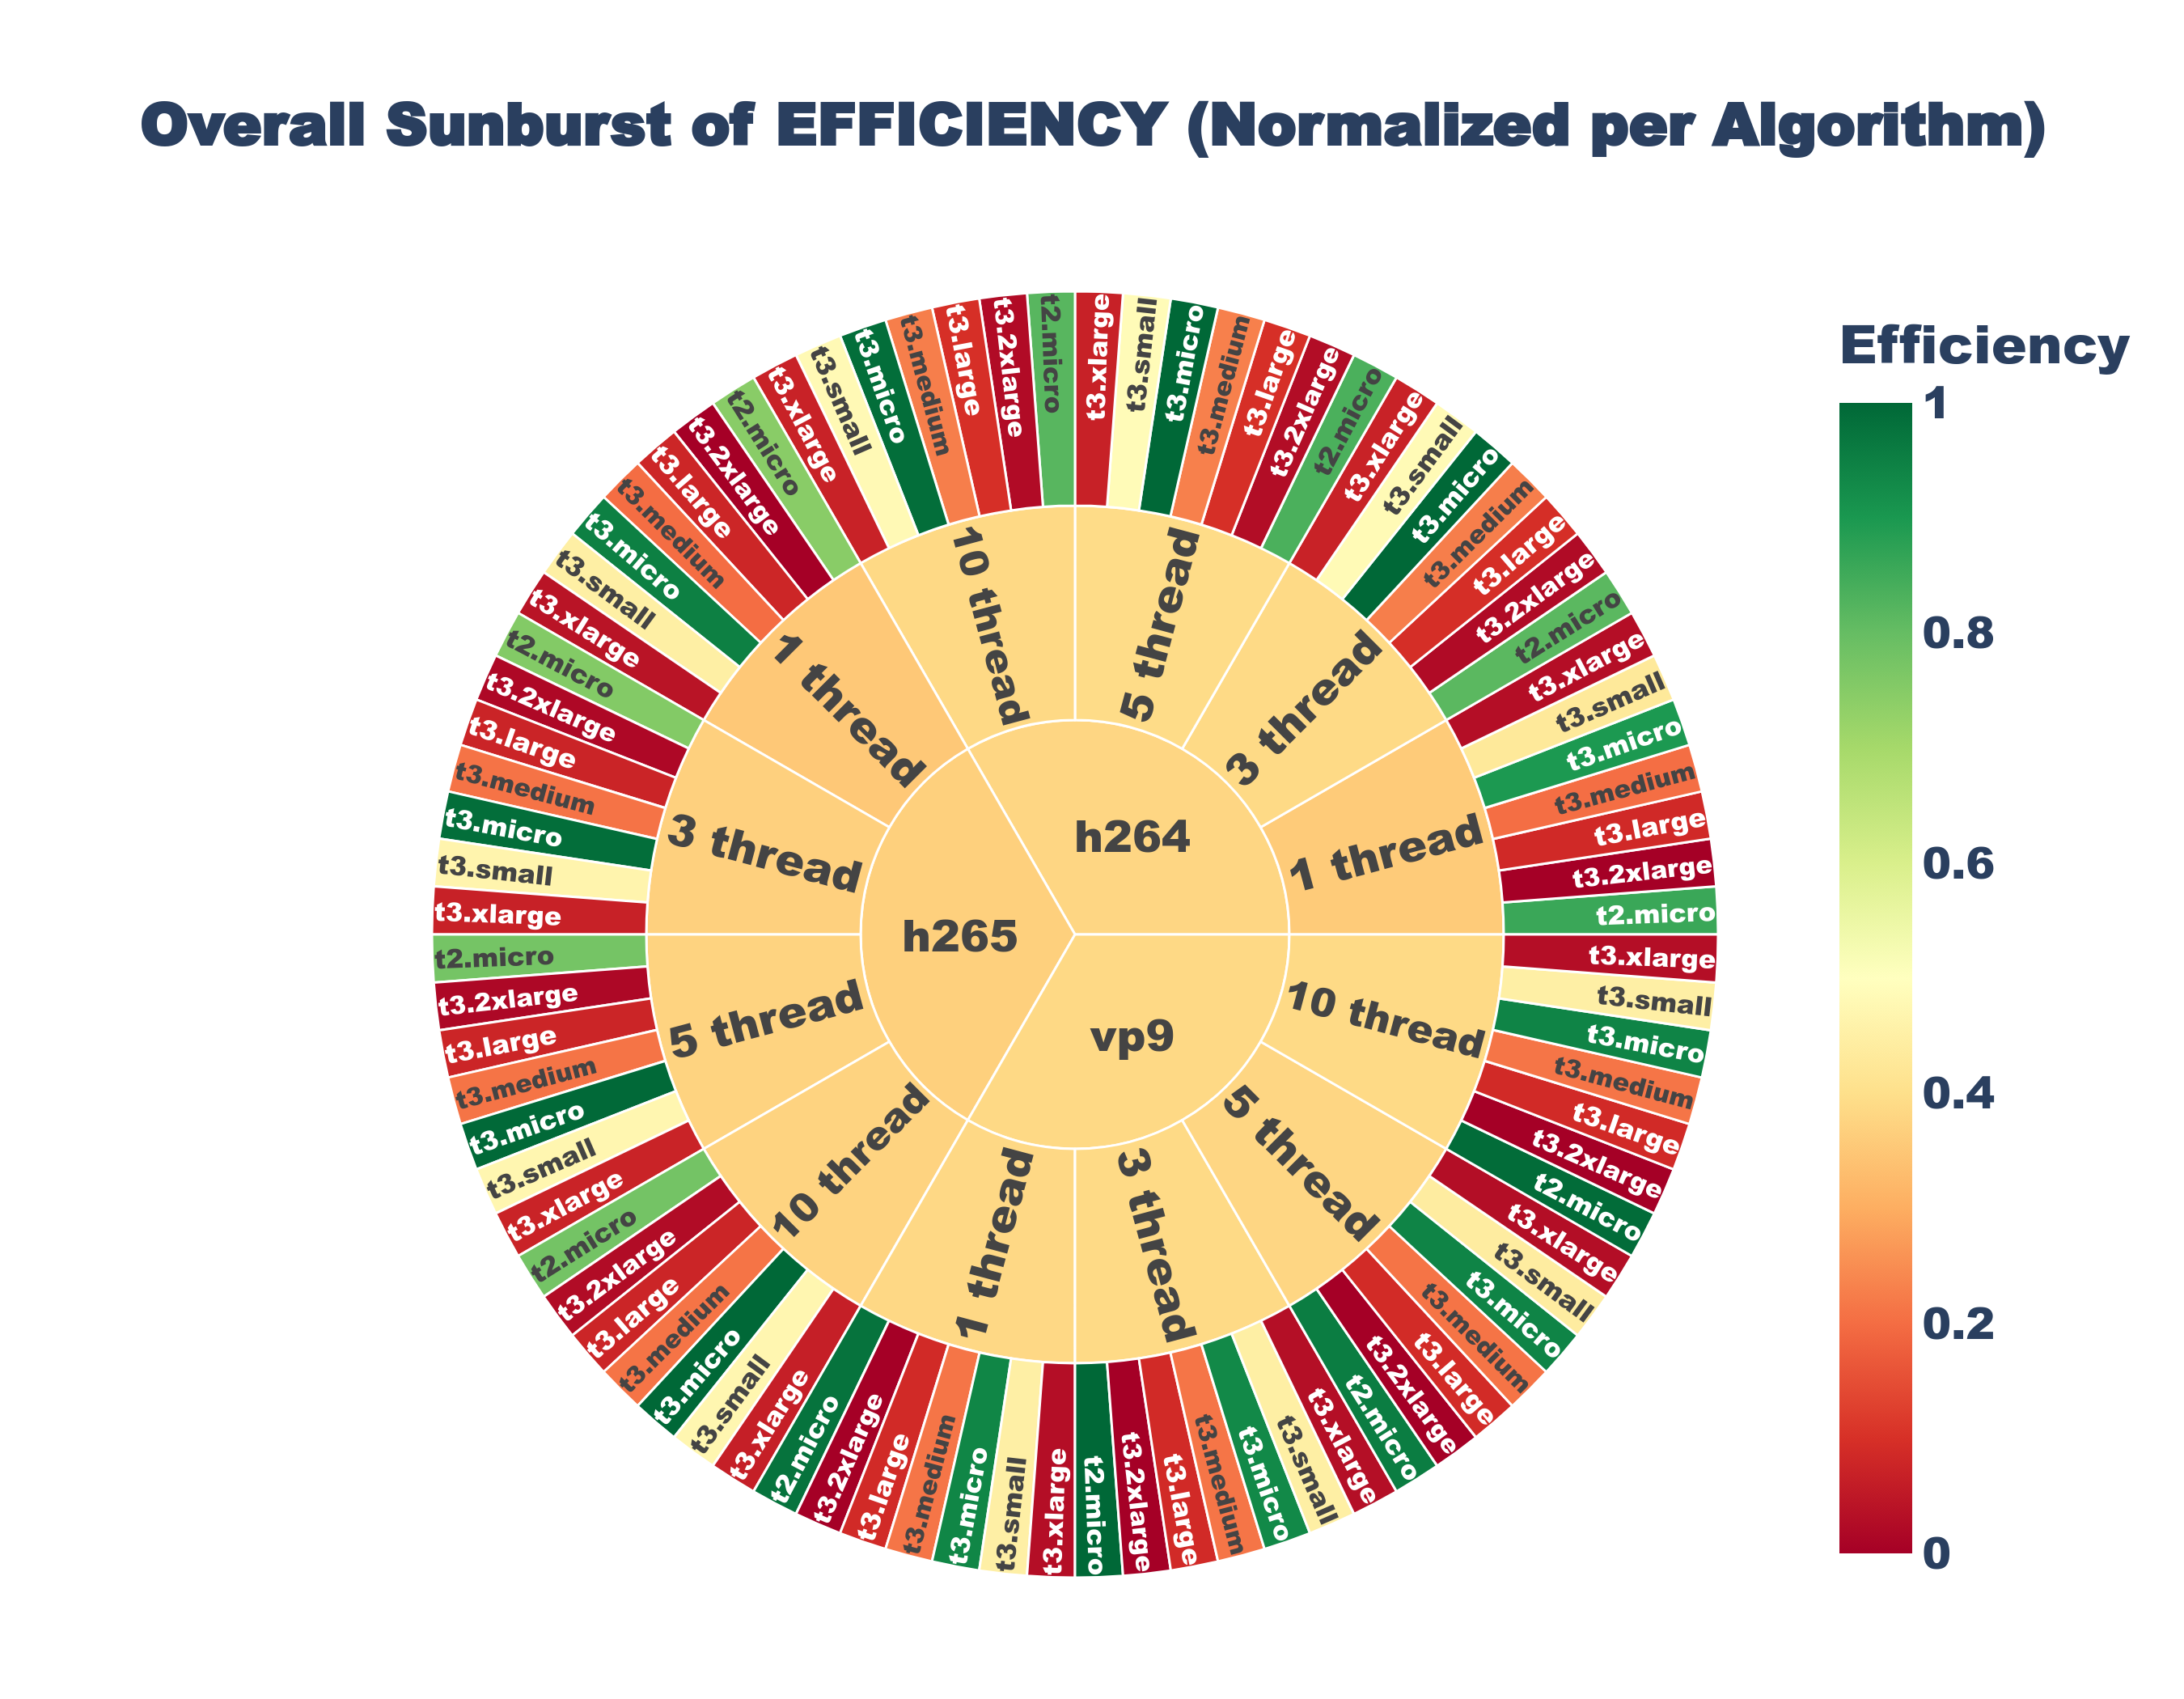
\includegraphics[width=0.8\textwidth]{graphs/sunburst_efficiency_normalized_overall.pdf}
		\caption{Hierarchical visualization of encoding efficiency across all experimental configurations. The sunburst diagram organizes results with color intensity and segment size proportional to normalized efficiency values within each algorithmic category.}
		\label{fig:sunburst_efficiency_normalized_overall}
	\end{figure*}
	
	
	
	

	
	Hierarchical efficiency overview is provided in Figure~\ref{fig:sunburst_efficiency_normalized_overall}, presenting a normalized Sunburst chart that enables clear comparison of instance and thread configurations within each algorithmic context.
	

	Algorithm-specific efficiency analysis appears in Figures~\ref{fig:h264_heatmap}, \ref{fig:h265_heatmap} and \ref{fig:vp9_heatmap}, visualizing median efficiency through heatmaps that correlate thread count with instance type. Color intensity represents cost-efficiency, enabling identification of optimal configurations.
	
	% Figura H.264 Efficiency Heatmap
	\begin{figure}[H]
		\centering
		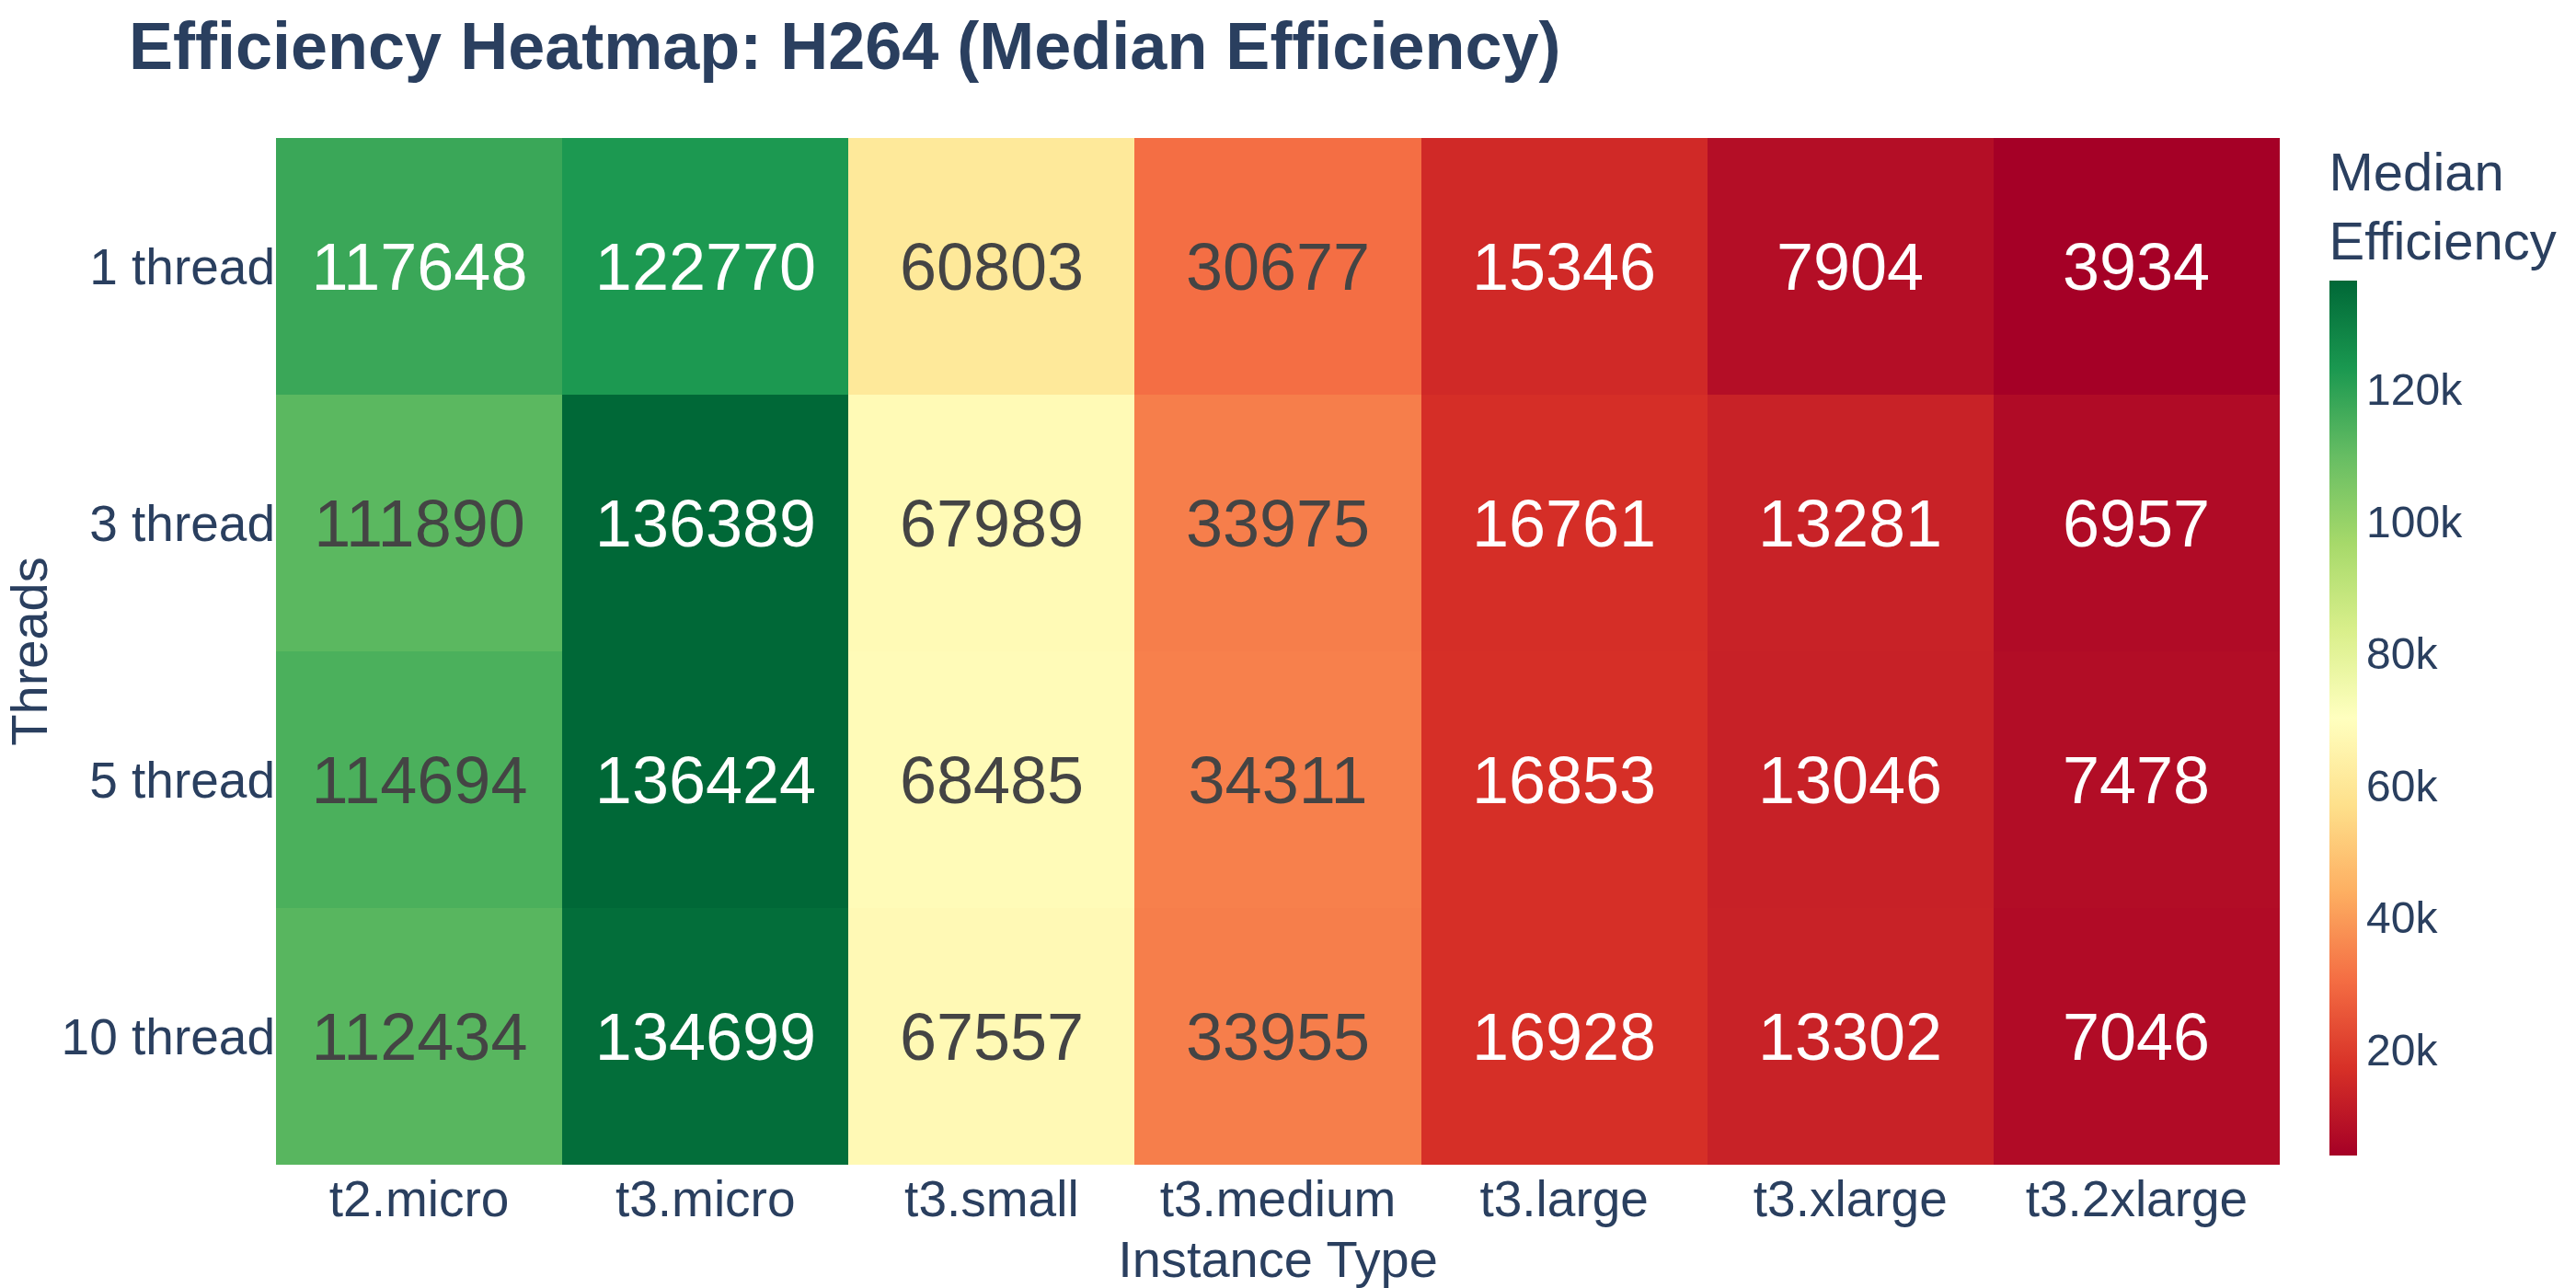
\includegraphics[width=0.9\columnwidth,keepaspectratio]{graphs/heatmap_efficiency_h264.png}
		\caption{H.264 Codec Efficiency: Heatmap visualization correlating thread count (vertical) with instance type (horizontal).}
		\label{fig:h264_heatmap}
	\end{figure}
	
	% Figura H.265 Efficiency Heatmap
	\begin{figure}[H]
		\centering
		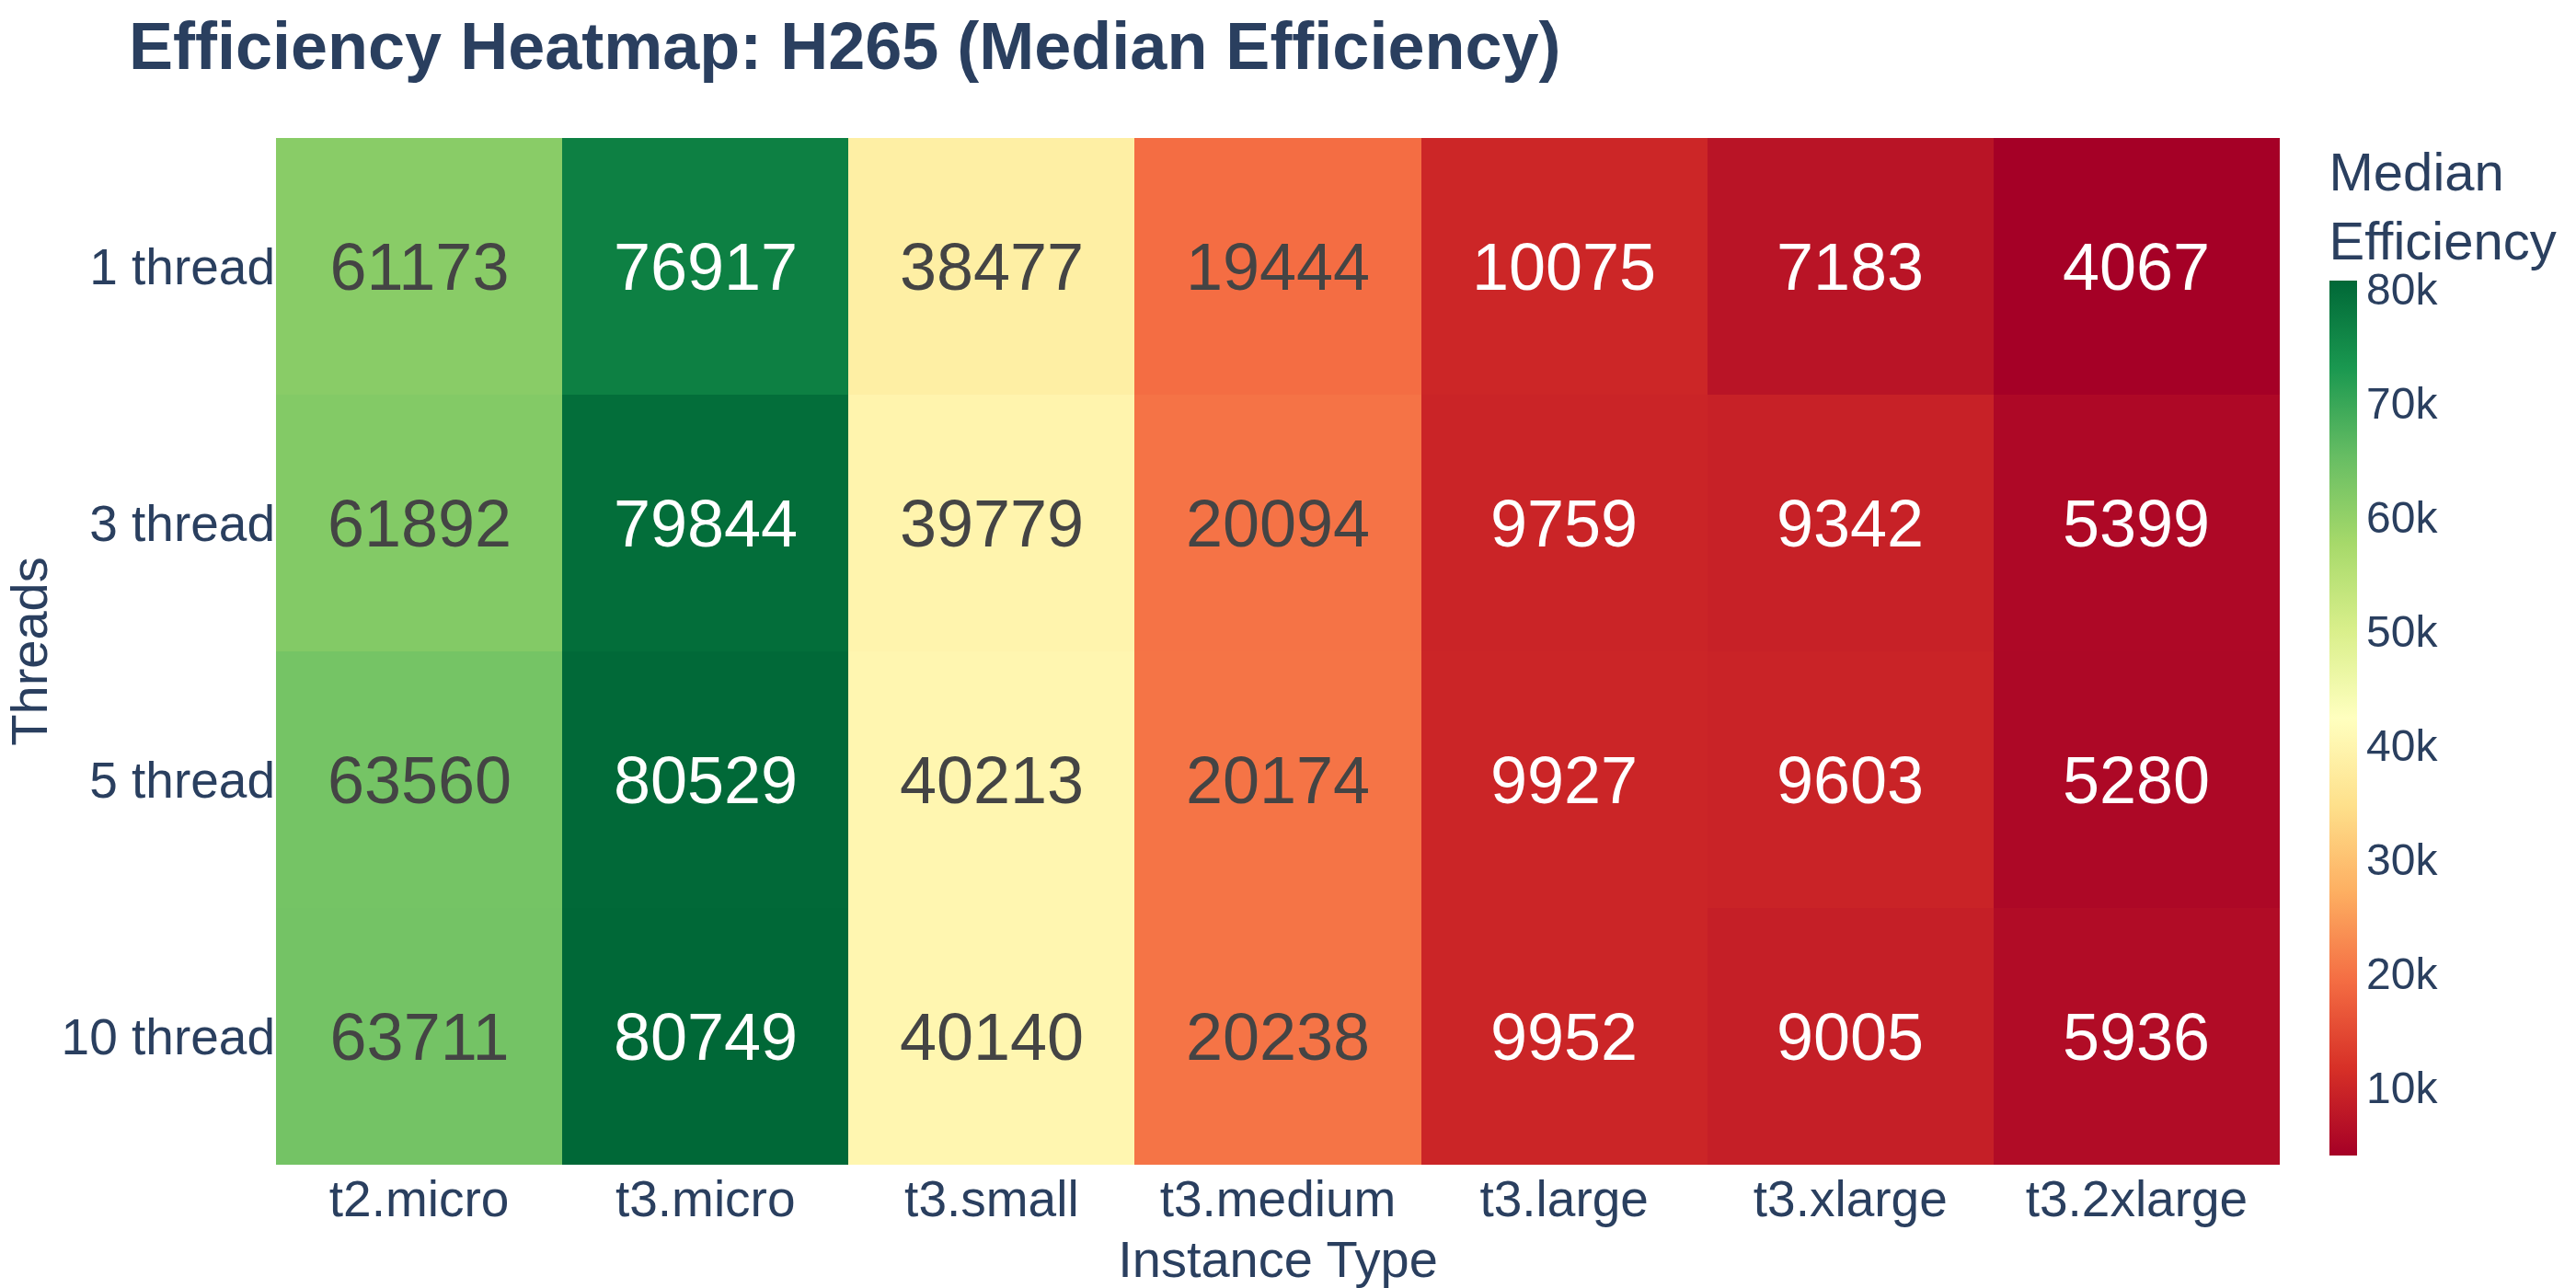
\includegraphics[width=0.9\columnwidth,keepaspectratio]{graphs/heatmap_efficiency_h265.png}
		\caption{H.265 Codec Efficiency: Heatmap visualization correlating thread count (vertical) with instance type (horizontal). Brighter colors indicate higher cost-efficiency scores.}
		\label{fig:h265_heatmap}
	\end{figure}
	
	
	
	
		
	% Figura VP9 Efficiency Heatmap
	\begin{figure}[!h]
		\centering
		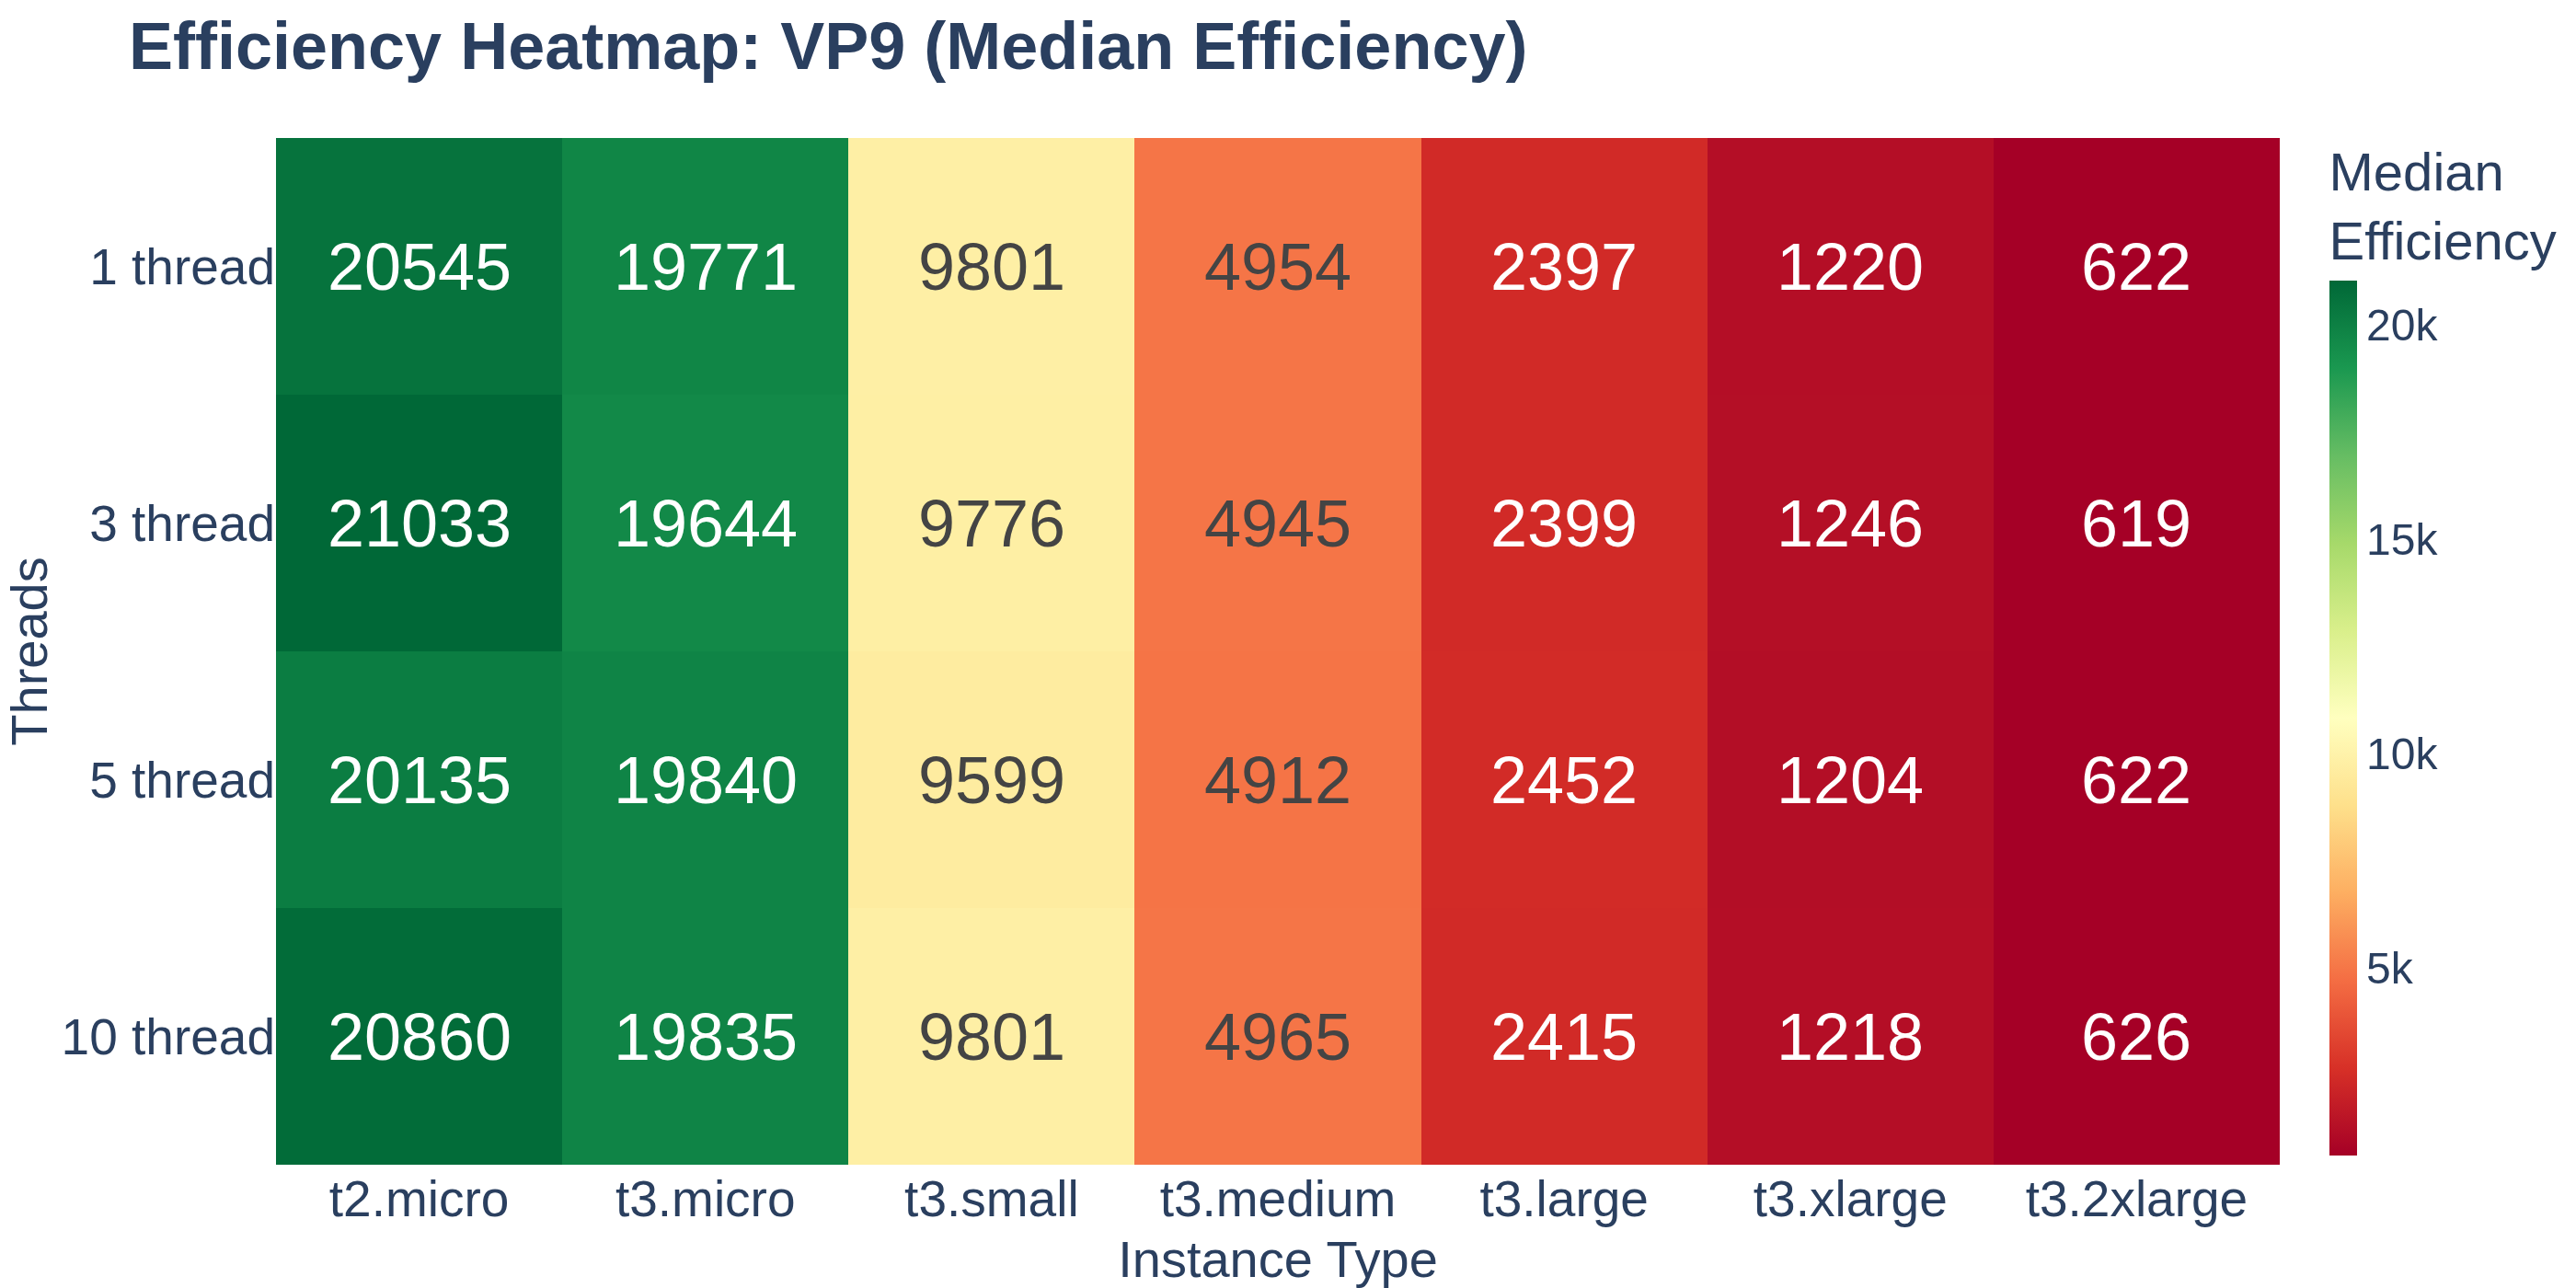
\includegraphics[width=0.98\columnwidth,keepaspectratio]{graphs/heatmap_efficiency_vp9.png}
		\caption{VP9 Codec Efficiency: Heatmap visualization correlating thread count (vertical) with instance type (horizontal). Brighter colors indicate higher cost-efficiency scores.}
		\label{fig:vp9_heatmap}
	\end{figure}
	
	\subsection{Phase 3 Results: Horizontal vs. Vertical Scaling Analysis}
	\label{results-phase3}
	
	Building upon findings that identified \texttt{t3.micro} as the optimal "Sweet Spot" (most cost-effective instance architecture) for H.264 compression, we conducted a comparative analysis of scaling strategies using a 10-minute H.264 video workload. While Phase 2 demonstrated that encoding times and specific efficiency curves vary significantly across different codecs (e.g., VP9 requires substantially more compute than H.264), we isolated H.264 for this scaling case study to control algorithmic variables and strictly evaluate architectural provisioning dynamics. Three architectural approaches were evaluated: horizontal scaling employing ten \texttt{t3.micro} instances (\$$0.0104$/h each, totaling \$$0.104$/h) processing one-minute segments in parallel; vertical scaling utilizing a single \texttt{t3.2xlarge} instance (\$$0.3328$/h) processing the complete video; and a baseline configuration with one \texttt{t3.micro} instance processing the video sequentially. Although a cost-equivalent vertical comparison for the 10-node cluster would be the \texttt{t3.large} (\$$0.0832$/h), we deliberately selected the \texttt{t3.2xlarge} to represent the absolute \textit{maximum performance limit} of the instance family. This comparison demonstrates that horizontal clustering does not merely rival cost-equivalent hardware, but successfully outperforms the fastest vertical node available on the market for that tier.
	
	\subsubsection{Two-Phase Analysis Results}
	
	The investigation employed a two-phase methodology to isolate provisioning overhead from computational performance. Phase 3.1 implemented dynamic provisioning with standard Ubuntu images and post-deployment dependency installation. This approach revealed that setup activities consumed 56.1-75.9\% of total processing time across configurations. Vertical scaling completed the workload in 3.04 minutes, outperforming horizontal scaling (3.28 minutes) by 7.9\%. Despite this performance differential, the horizontal approach demonstrated substantial cost advantages, operating at \$0.00568 compared to \$0.01687 for vertical scaling—a 66.3\% reduction.
	
	Phase 3.2 employed optimized provisioning through custom Amazon Machine Images (AMIs) with pre-installed dependencies. This optimization yielded transformative results: horizontal scaling achieved 1.45 minutes total processing time, representing a 55.9\% improvement over Phase 3.1 and 1.28× faster execution than vertical scaling (1.85 minutes). Costs were reduced by 55.8\% to \$0.00251, achieving 75.5\% cost reduction compared to vertical scaling. Setup time decreased from 2.30 minutes to 0.98 minutes, a 57.4\% reduction in absolute provisioning overhead.
	
	\subsubsection{Analysis and Validation}
	
	It is important to clarify the definition of \textit{Effective Encoding Time} in the parallel context. For a single \texttt{t3.micro} processing the 10-minute video serially (Phase 3.2), raw computation takes 1.78 minutes. When divided across 10 instances, the theoretical raw computation per instance should be $\approx 0.178$ minutes. However, the reported parallel Effective Encoding Time is 0.47 minutes. This study implements a lightweight, state-less orchestration architecture to enforce strict isolation of cloud provisioning phenomena. Rather than relying on managed queues (SQS) or blob storage (S3) which introduce third-party variable latency, orchestration is driven by a localized Python controller. The controller pre-segments the source video using FFmpeg, synchronously provisions the target EC2 instances via the AWS API (\texttt{boto3}), and establishes parallel SSH/SFTP tunnels to dispatch the segments, execute the encoding natively via the custom AMI, and retrieve the compressed outputs. Consequently, our Effective Time metric perfectly encapsulates the raw FFmpeg computation \textit{plus} these intrinsic network I/O transfers, while \textit{Setup Overhead} strictly bounds the API-to-Running cloud provisioning latency (from creation request until SSH daemon accessibility).
	
	Table~\ref{tab:unified_case_study} presents comparison data across optimization phases, demonstrating that properly optimized horizontal scaling achieves superior performance and cost-efficiency. Figure~\ref{fig:ami_comparison} further illustrates that horizontal scaling achieves superior performance and cost-efficiency when provisioning overhead is minimized through AMI optimization.
	
	\begin{table*}[!htpb]
		\centering
		\caption{Comparison of scaling strategies across optimization phases for Burstable (T) Family (Time values include $\pm$3\% derived 95\% CI margin of error)}
		\label{tab:unified_case_study}
		\begin{tabular*}{\textwidth}{l @{\extracolsep{\fill}} | cc | cc | cc}
			\toprule
			& \multicolumn{2}{c|}{\textbf{Serial (1x t3.micro)}} & \multicolumn{2}{c|}{\textbf{Parallel (10x t3.micro)}} & \multicolumn{2}{c}{\textbf{Serial (1x t3.2xlarge)}} \\
			\cmidrule(lr){2-3} \cmidrule(lr){4-5} \cmidrule(lr){6-7}
			\textbf{Metric} & \textbf{Phase 3.1} & \textbf{Phase 3.2} & \textbf{Phase 3.1} & \textbf{Phase 3.2} & \textbf{Phase 3.1} & \textbf{Phase 3.2} \\
			\midrule
			Total Time (min)          & 4.03 $\pm$ 0.12  & 2.80 $\pm$ 0.08  & 3.28 $\pm$ 0.10 & \textbf{1.45 $\pm$ 0.04} & 3.04 $\pm$ 0.09 & 1.85 $\pm$ 0.06 \\
			Setup Overhead (min)      & 2.26  & 1.02  & 2.30 & \textbf{0.98} & 2.31 & 1.11 \\
			Setup Overhead (\%)       & 56.1\% & 36.5\% & 70.2\% & 67.6\% & 75.9\% & 59.7\% \\
			Effective Encoding Time (min) & 1.77  & 1.78  & 0.97 & 0.47 & \textbf{0.73} & 0.74 \\
			\midrule
			Total Cost (USD)          & \$0.00070 & \$0.00048 & \$0.00568 & \textbf{\$0.00251} & \$0.01687 & \$0.01026 \\
			Cost per Minute Video     & \$0.000070 & \$0.000048 & \$0.000568 & \textbf{\$0.000251} & \$0.001687 & \$0.001026 \\
			\midrule \midrule
			\textbf{Time Improvement} & \multicolumn{2}{c|}{30.5\%} & \multicolumn{2}{c|}{\textbf{55.9\%}} & \multicolumn{2}{c}{39.1\%} \\
			\textbf{Cost Reduction}   & \multicolumn{2}{c|}{31.4\%} & \multicolumn{2}{c|}{\textbf{55.8\%}} & \multicolumn{2}{c}{39.2\%} \\
			\bottomrule
		\end{tabular*}
	\end{table*}
	
    \begin{table*}[!htpb]
        \centering
        \caption{Comparison of scaling strategies across optimization phases for General Purpose (M) and Compute Optimized (C) Families (Time values include $\pm$3\% derived 95\% CI margin of error)}
        \label{tab:unified_case_study_mc}
        \begin{tabular*}{\textwidth}{l @{\extracolsep{\fill}} | cc | cc | cc}
            \toprule
            \multicolumn{7}{c}{\textbf{General Purpose (M) Family}} \\
            \midrule
            & \multicolumn{2}{c|}{\textbf{Serial (1x m5.large)}} & \multicolumn{2}{c|}{\textbf{Parallel (10x m5.large)}} & \multicolumn{2}{c}{\textbf{Serial (1x m5.4xlarge)}} \\
            \cmidrule(lr){2-3} \cmidrule(lr){4-5} \cmidrule(lr){6-7}
            \textbf{Metric} & \textbf{Phase 3.1} & \textbf{Phase 3.2} & \textbf{Phase 3.1} & \textbf{Phase 3.2} & \textbf{Phase 3.1} & \textbf{Phase 3.2} \\
            \midrule
            Total Time (min)          & 3.46 $\pm$ 0.10  & 2.90 $\pm$ 0.09  & 3.63 $\pm$ 0.11 & \textbf{1.35 $\pm$ 0.04} & 2.33 $\pm$ 0.07 & 1.65 $\pm$ 0.05 \\
            Setup Overhead (min)      & 1.56  & 0.96  & 2.50 & \textbf{0.90} & 1.74 & 0.95 \\
            Setup Overhead (\%)       & 45.1\% & 33.1\% & 68.9\% & 66.7\% & 74.7\% & 57.6\% \\
            Effective Encoding Time (min) & 1.90  & 1.94  & 1.13 & 0.45 & \textbf{0.59} & 0.70 \\
            \midrule
            Total Cost (USD)          & \$0.00554 & \$0.00464 & \$0.05808 & \textbf{\$0.02160} & \$0.02982 & \$0.02112 \\
            Cost per Minute Video     & \$0.00055 & \$0.00046 & \$0.00581 & \textbf{\$0.00216} & \$0.00298 & \$0.00211 \\
            \midrule \midrule
            \textbf{Time Improvement} & \multicolumn{2}{c|}{16.2\%} & \multicolumn{2}{c|}{\textbf{62.8\%}} & \multicolumn{2}{c}{29.2\%} \\
            \textbf{Cost Reduction}   & \multicolumn{2}{c|}{16.2\%} & \multicolumn{2}{c|}{\textbf{62.8\%}} & \multicolumn{2}{c}{29.2\%} \\
            
            \midrule
            \multicolumn{7}{c}{\textbf{Compute Optimized (C) Family}} \\
            \midrule
            & \multicolumn{2}{c|}{\textbf{Serial (1x c5.large)}} & \multicolumn{2}{c|}{\textbf{Parallel (10x c5.large)}} & \multicolumn{2}{c}{\textbf{Serial (1x c5.4xlarge)}} \\
            \cmidrule(lr){2-3} \cmidrule(lr){4-5} \cmidrule(lr){6-7}
            \textbf{Metric} & \textbf{Phase 3.1} & \textbf{Phase 3.2} & \textbf{Phase 3.1} & \textbf{Phase 3.2} & \textbf{Phase 3.1} & \textbf{Phase 3.2} \\
            \midrule
            Total Time (min)          & 3.21 $\pm$ 0.10  & 2.64 $\pm$ 0.08  & 3.52 $\pm$ 0.11 & \textbf{1.31 $\pm$ 0.04} & 2.13 $\pm$ 0.06 & 1.54 $\pm$ 0.05 \\
            Setup Overhead (min)      & 1.55  & 0.98  & 2.50 & \textbf{0.90} & 1.54 & 0.95 \\
            Setup Overhead (\%)       & 48.3\% & 37.1\% & 71.0\% & 68.7\% & 72.3\% & 61.7\% \\
            Effective Encoding Time (min) & 1.66  & 1.66  & 1.02 & 0.41 & \textbf{0.59} & 0.59 \\
            \midrule
            Total Cost (USD)          & \$0.00455 & \$0.00374 & \$0.04986 & \textbf{\$0.01856} & \$0.02414 & \$0.01745 \\
            Cost per Minute Video     & \$0.00045 & \$0.00037 & \$0.00499 & \textbf{\$0.00186} & \$0.00241 & \$0.00175 \\
            \midrule \midrule
            \textbf{Time Improvement} & \multicolumn{2}{c|}{17.8\%} & \multicolumn{2}{c|}{\textbf{62.8\%}} & \multicolumn{2}{c}{27.7\%} \\
            \textbf{Cost Reduction}   & \multicolumn{2}{c|}{17.8\%} & \multicolumn{2}{c|}{\textbf{62.8\%}} & \multicolumn{2}{c}{27.7\%} \\
            \bottomrule
        \end{tabular*}
    \end{table*}
	
	\begin{figure}[!ht]
		\centering
		
\includegraphics[width=0.5\textwidth]{graphs/comparison_time_cost_dual_axis.png}
		\caption{Performance and cost comparison between dynamic provisioning (Phase 3.1) and optimized provisioning (Phase 3.2). The dual-axis visualization demonstrates that horizontal scaling achieves superior performance and cost-efficiency when provisioning overhead is minimized through AMI optimization.}
		\label{fig:ami_comparison}
	\end{figure}
	
	\subsubsection{Cross-Family Scaling Validation}
	
	To validate the universality of the horizontal scaling advantage, we extended the optimized provisioning strategy (Phase 3.2) to General Purpose (M) and Compute Optimized (C) families. Table \ref{tab:cross_family_scaling} presents the comparative results.
	
	\begin{table}[h]
		\centering
		\caption{Scaling Strategy Comparison across Instance Families (Phase 3.2). Time values include $\pm$3\% margin of error.}
		\label{tab:cross_family_scaling}
		\resizebox{\columnwidth}{!}{
			\begin{tabular}{|l|l|c|c|c|}
				\hline
				\textbf{Family} & \textbf{Strategy} & \textbf{Total Time (min)} & \textbf{Total Cost (\$)} & \textbf{Speedup vs Vertical} \\
				\hline
				\textbf{Burstable (T)} & Horizontal (10x t3.micro) & \textbf{1.45 $\pm$ 0.04} & \textbf{0.0025} & \textbf{1.28x} \\
				\textbf{(Sweet Spot)} & Vertical (1x t3.2xlarge) & 1.85 $\pm$ 0.06 & 0.0102 & - \\
				\hline
				\textbf{General (M)} & Horizontal (10x m5.large) & \textbf{1.35 $\pm$ 0.04} & 0.0215 & \textbf{1.22x} \\
				& Vertical (1x m5.4xlarge) & 1.65 $\pm$ 0.05 & 0.0211 & - \\
				\hline
				\textbf{Compute (C)} & Horizontal (10x c5.large) & \textbf{1.31 $\pm$ 0.04} & 0.0185 & \textbf{1.17x} \\
				\textbf{(Speed King)} & Vertical (1x c5.4xlarge) & 1.54 $\pm$ 0.05 & 0.0174 & - \\
				\hline
			\end{tabular}
		}
	\end{table}

	The results confirm that the performance advantage of optimized horizontal scaling is widely applicable. As detailed in Table \ref{tab:unified_case_study_mc}, for the M-family, the horizontal cluster achieved a 1.22x speedup (1.35 min vs 1.65 min). For the C-family (Table \ref{tab:unified_case_study_mc}), the cluster achieved the fastest overall time of 1.31 minutes (1.17x speedup vs 1.54 min).
	
	However, unlike the T-family which delivered a massive 75\% cost reduction, horizontal scaling for the M and C families proved marginally more expensive than their vertical counterparts. The M-family cluster cost \$0.0215 compared to \$0.0211 for vertical, and the C-family cluster cost \$0.0185 versus \$0.0174. In these specific families, horizontal clustering shifts from being a cost-saving strategy to a \textit{performance-maximizing} strategy.
	
	Crucially, this data refutes the assumption that vertical scaling is the only avenue for high-performance tasks. Even for Compute Optimized workloads, a cluster of smaller instances (c5.large) outperformed the processing speed of the largest vertical node (c5.4xlarge) when provisioning overhead was minimized, albeit at a negligible cost premium of just \$0.0004 (\textasciitilde0.4 cents) per 10-minute video. While the T-family offers extreme economic efficiency, the M and C families demonstrate that horizontal scaling provides a viable temporal advantage for time-critical applications.
	
	\begin{figure}[!ht]
		\centering
		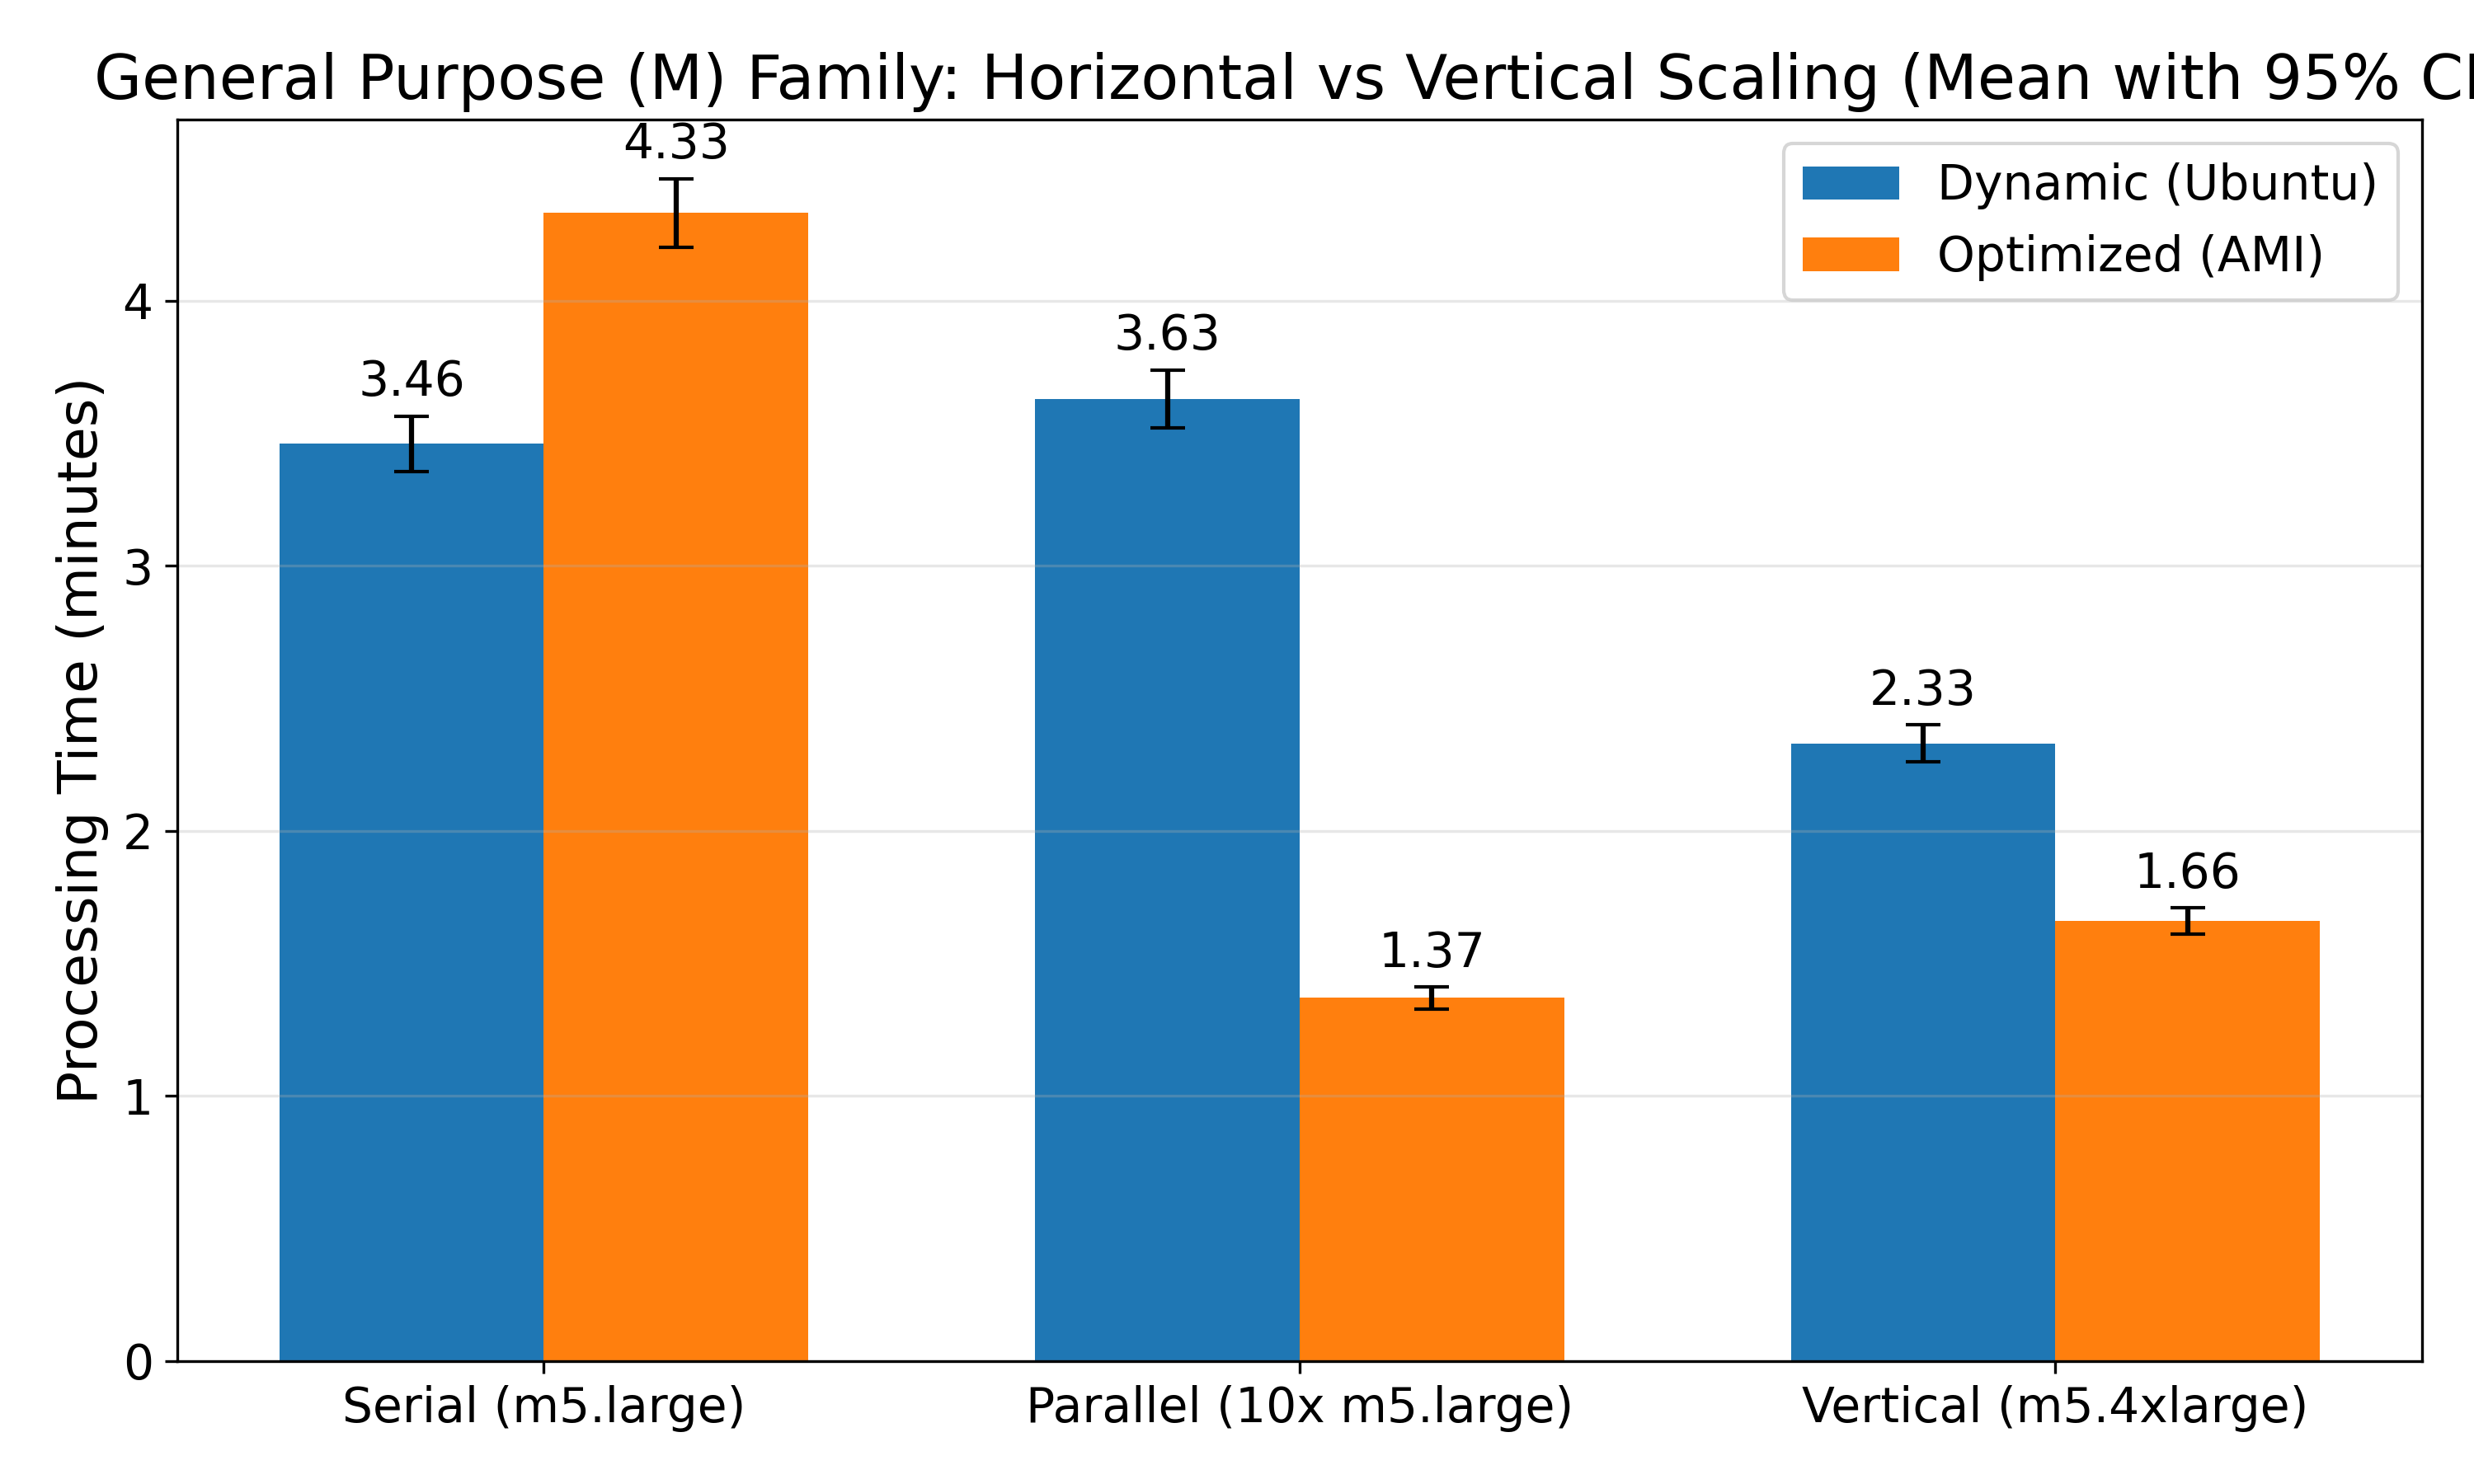
\includegraphics[width=0.45\textwidth]{graphs/scaling_comparison_m_family.png}
		\caption{Performance and cost scaling comparison for General Purpose (M) family instances, demonstrating consistent horizontal scaling speedup capabilities.}
		\label{fig:scaling_m_family}
	\end{figure}
	
	\begin{figure}[!ht]
		\centering
		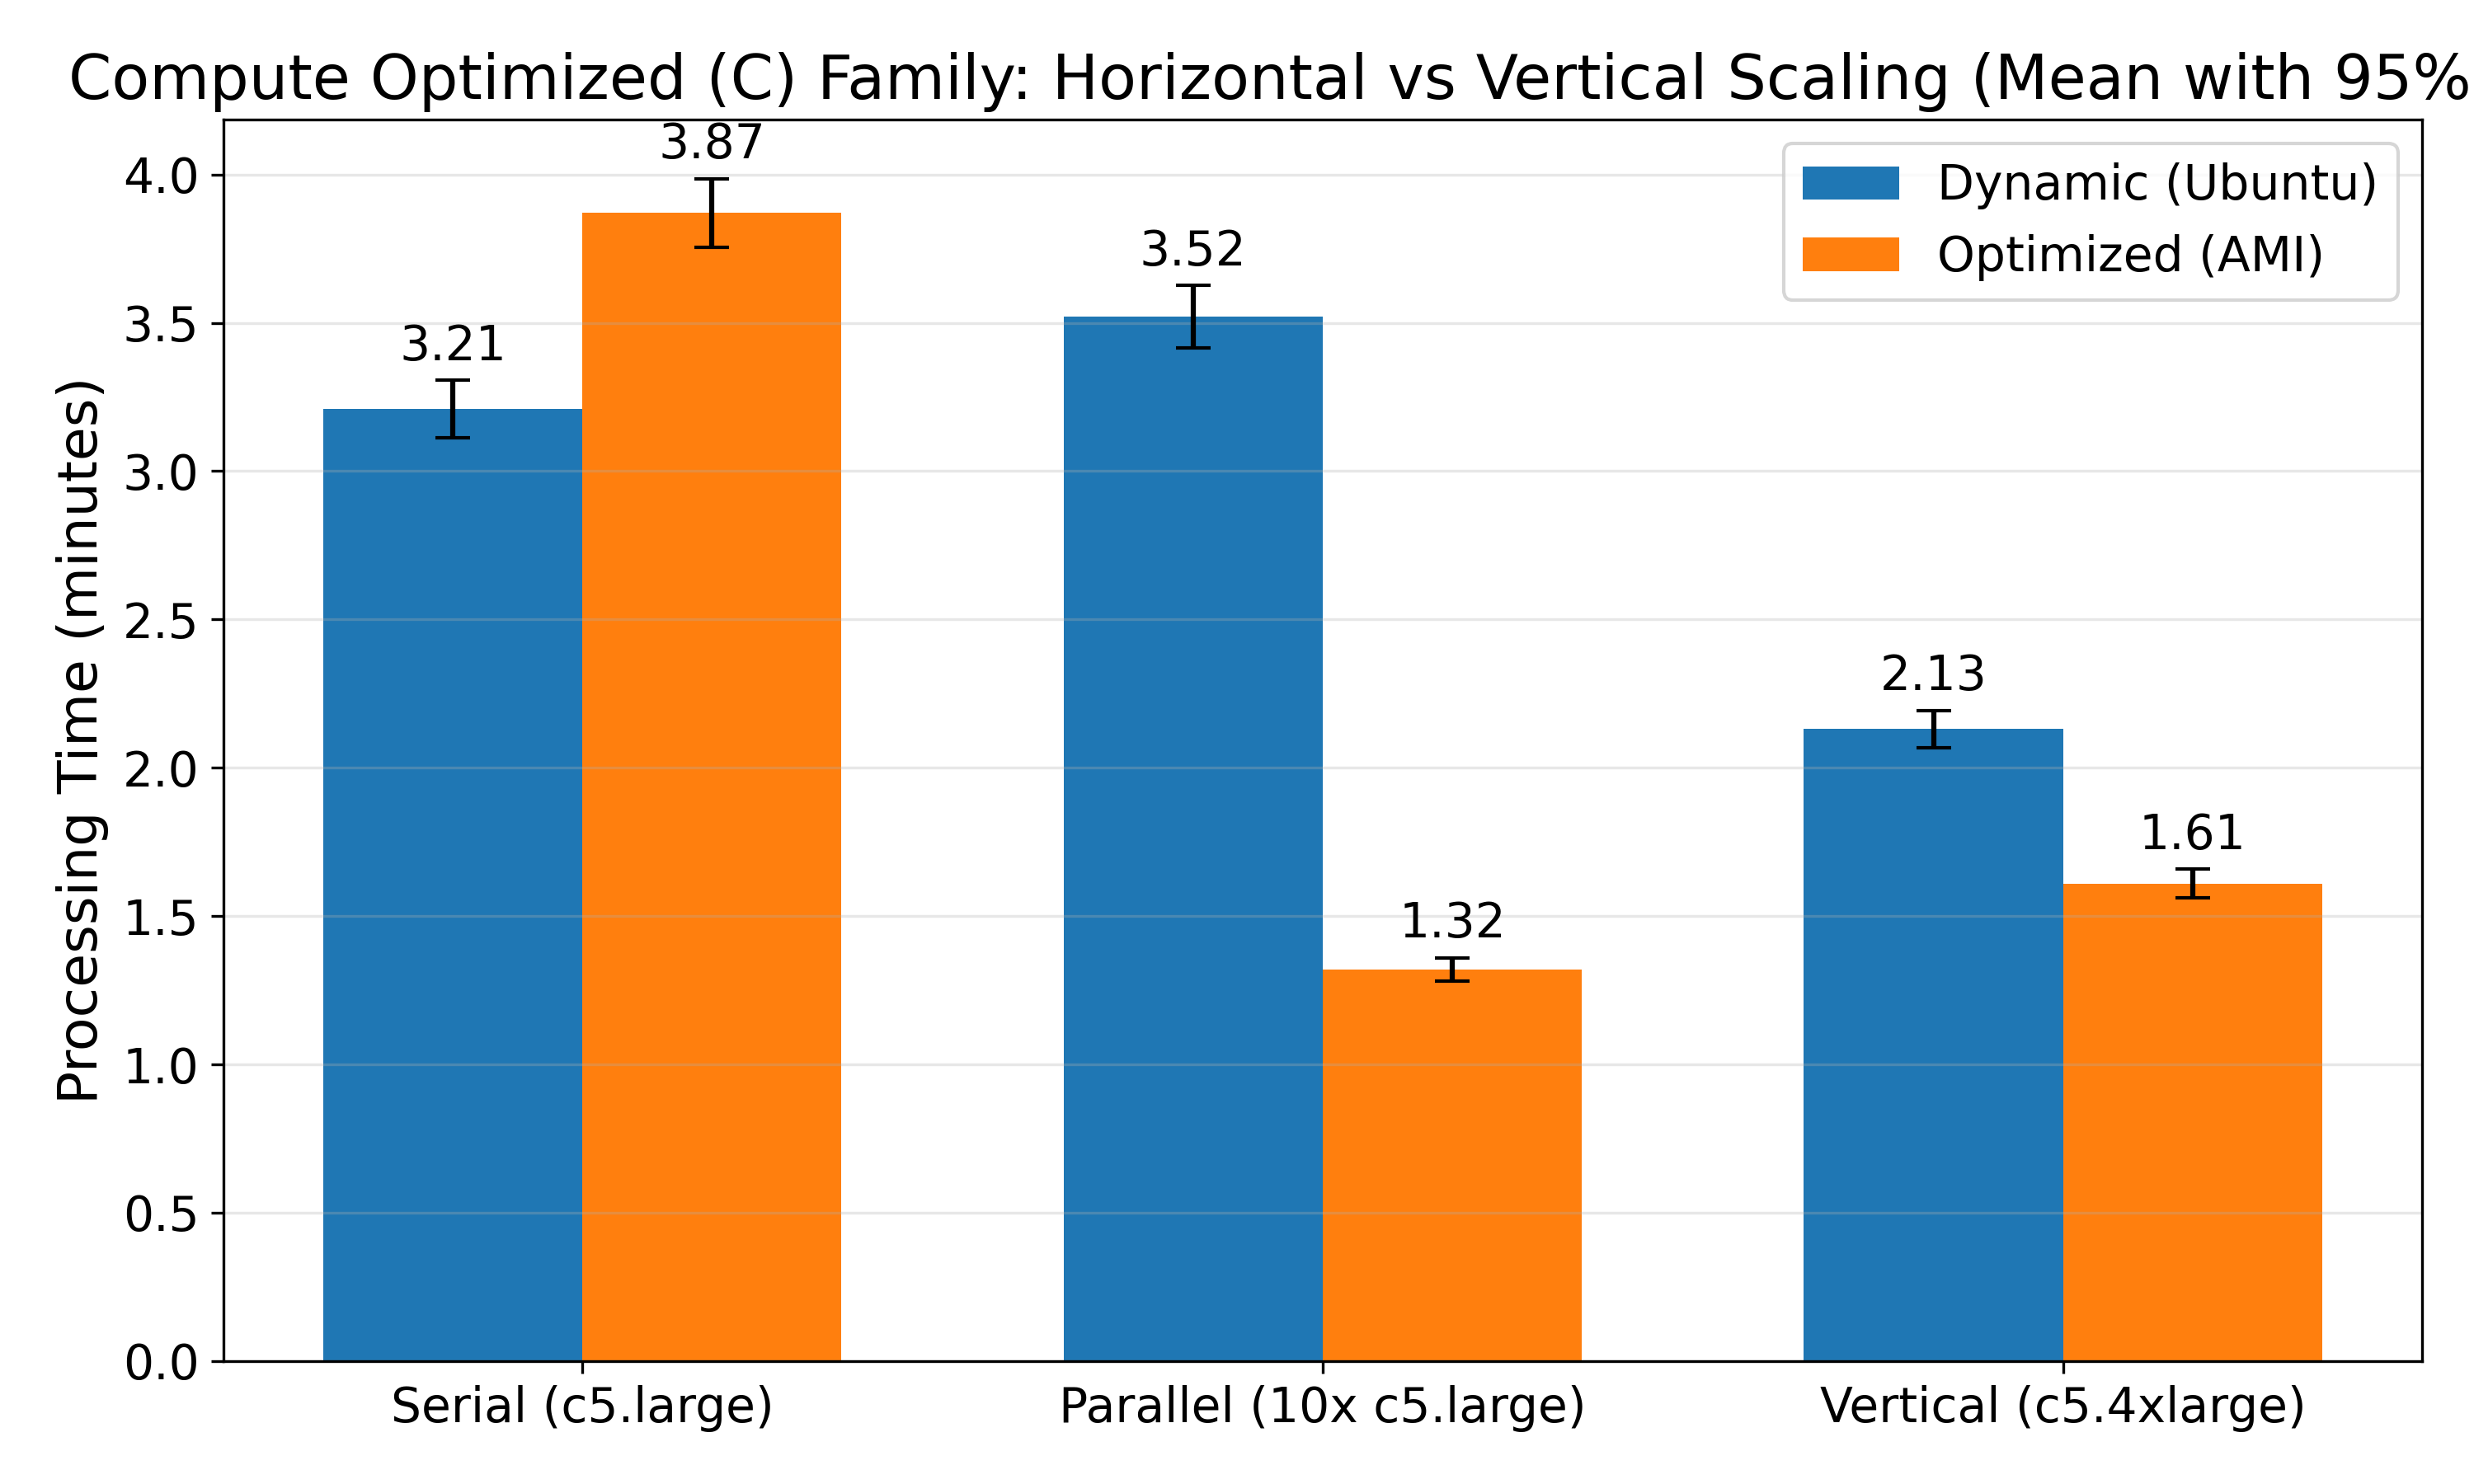
\includegraphics[width=0.45\textwidth]{graphs/scaling_comparison_c_family.png}
		\caption{Performance and cost scaling comparison for Compute Optimized (C) family instances, challenging the necessity of vertical scaling for high-performance computing.}
		\label{fig:scaling_c_family}
	\end{figure}
	\subsubsection{Methodological Validation}
	
	The experimental design provides robust validation through multiple approaches: controlled comparison of identical workloads across scaling strategies; precise quantification of provisioning overhead (70.2\% of total time in unoptimized deployments); statistical confidence from multiple experimental runs ($n=30$ for Phase 2 benchmarks, $n=10$ for Phase 3 macro-architecture configurations); and practical relevance through realistic workload (10-minute video) and applicable optimization strategy (custom AMIs).
	
	The results demonstrate that horizontal scaling's theoretical advantages can be realized when operational bottlenecks are addressed. The documented 75.5\% cost reduction (T-family) and universal speedup (all families) provide compelling evidence for re-evaluating conventional vertical scaling approaches for video encoding workloads in cloud environments.
	
\section{Discussion and Threats to Validity}
\label{limitations}

While our findings advocate for optimized horizontal scaling, several operational constraints and validity threats must be acknowledged when generalizing these results.

\subsection{Internal Validity}
\textbf{Burstable Instance Sustainability and CPU Credits:} T-family instances operate in Unlimited mode by default, allowing immediate 100\% CPU bursts but risking surcharge fees upon credit depletion. However, a newly launched \texttt{t3.micro} receives 30 launch CPU credits upon boot. Our 1-minute 100\% CPU encoding burst consumes approximately 2 credits. Therefore, our ephemeral architectural pattern (spawn, encode, terminate) completely absorbs the workload within the free launch balance, guaranteeing zero Unlimited mode surcharges. While sustained 24/7 encoding on a persistent node would eventually incur fees, our methodology is inherently built for discrete batch workloads (e.g., scheduled transcoding, pipelines) where short-lived instances bypass credit exhaustion entirely.

\textbf{Cost Scope Constraints:} This study exclusively evaluates compute costs, as they represent the dominant expense in transcoding pipelines. Infrastructure costs such as storage (EBS) and data transfer scale linearly with data volume regardless of the instance type used, rendering our relative efficiency comparisons mathematically sound. Additionally, the use of open-source software (Ubuntu, FFmpeg) eliminates licensing overhead, a critical prerequisite for cost-efficient horizontal scaling.

\subsection{External \& Construct Validity}
\textbf{Generalizability:} Experiments were conducted using a single AWS region (us-east-1) and x86 architectures. Phase 3 scaling results are validated exclusively for H.264; codec-specific provisioning behavior for computationally heavier codecs such as H.265 and VP9 remains an open research question. Furthermore, while our core mechanism of eliminating provisioning overhead applies universally, absolute economics will shift. Regional pricing parity varies heavily (e.g., the South America \texttt{sa-east-1} region is typically $\sim$50\% more expensive than \texttt{us-east-1}). Future research should map these shifts against ARM-based instances (e.g., AWS Graviton) and GPU-accelerated environments.

\textbf{Sensitivity and Architectural Constraints:} This scaling study applies 60-second video chunks as a controlled baseline. To empirically quantify the impact of chunk size, we ran the same 10-minute H.264 workload with 30-second (20 nodes), 60-second (10 nodes), and 120-second (5 nodes) chunks across all three families. Total Time is measured end-to-end, comprising video segmentation, parallel AWS provisioning (boto3 waiter + 30s SSH readiness wait per instance), segment transfer, encoding, and output retrieval. Results are presented in Table \ref{tab:chunk_sensitivity}.

The findings reveal a clear sensitivity boundary: 30-second chunks across 20 nodes increase parallel provisioning coordination proportionally (20 bootstrap sequences instead of 10), which, for shorter encoding tasks, erodes the speedup advantage. Meanwhile, larger 120-second chunks with only 5 nodes reduce provisioning calls but fail to exploit parallelism sufficiently — the higher per-instance encoding burden dominates, and Total Time exceeds the vertical baseline across all families (speedup $<1.0\times$). The 60-second configuration uniquely balances these competing forces, delivering the best speedup in all three families. This empirical boundary underscores the need for dynamic chunk sizing algorithms in production VaaS pipelines.

\begin{table}[h]
	\centering
	\caption{Chunk Size Sensitivity Analysis (10-min H.264, Phase 3.2 AMI). Total Time is end-to-end wall-clock. Speedup vs each family's vertical baseline.}
	\label{tab:chunk_sensitivity}
	\resizebox{\columnwidth}{!}{
		\begin{tabular}{|l|l|c|c|}
			\hline
			\textbf{Family} & \textbf{Chunk Strategy} & \textbf{Total Time (min)} & \textbf{Speedup vs Vertical} \\
			\hline
			\multirow{3}{*}{Burstable (T)} & 30s (20x t3.micro) & 1.39 & 1.33x \\
			 & \textbf{60s (10x t3.micro)} & \textbf{1.45} & \textbf{1.28x} \\
			 & 120s (5x t3.micro) & 2.04 & 0.91x$^{*}$ \\
			\hline
			\multirow{3}{*}{General (M)} & 30s (20x m5.large) & 1.63 & 1.01x \\
			 & \textbf{60s (10x m5.large)} & \textbf{1.35} & \textbf{1.22x} \\
			 & 120s (5x m5.large) & 2.10 & 0.79x$^{*}$ \\
			\hline
			\multirow{3}{*}{Compute (C)} & 30s (20x c5.large) & 1.44 & 1.07x \\
			 & \textbf{60s (10x c5.large)} & \textbf{1.31} & \textbf{1.17x} \\
			 & 120s (5x c5.large) & 1.98 & 0.78x$^{*}$ \\
			\hline
			\multicolumn{4}{|l|}{\footnotesize $^{*}$ Speedup $< 1.0$ indicates horizontal cluster is \textit{slower} than vertical.} \\
			\hline
		\end{tabular}
	}
\end{table}
	
\section{Conclusion}
\label{conclusion}

This study demonstrates that the true barrier to cloud cost-efficiency for video encoding is not hardware limitation, but operational provisioning overhead. Our empirical analysis across diverse instance families—Burstable (T), General Purpose (M), and Compute Optimized (C)—quantified this bottleneck at approximately 70\% of total processing time in unmanaged environments.
 
By introducing a custom machine image (AMI) framework, we successfully eliminated this overhead. This optimization served as the critical prerequisite that unlocked horizontal scaling as a universally superior strategy. In fully optimized environments, clusters of ten \texttt{micro/large} instances consistently outperformed the raw processing speed of the largest available vertical instances (\texttt{2xlarge/4xlarge}) across all tested families. For the T-family specifically, this resulted in a 1.28× speedup combined with a massive 75.5\% cost reduction.

These findings challenge conventional resource allocation assumptions for Video-as-a-Service (VaaS) workloads. The results establish that removing cloud provisioning overhead shifts horizontal scaling from being merely an economic compromise to a definitive, performance-maximizing approach.

Future research should extend this overhead-elimination framework to GPU-accelerated instances, develop intelligent scaling systems that dynamically adjust cluster size based on variable chunk sensitivities, and explore fault-tolerant orchestration patterns for spot instances. This work provides a concrete foundation for VaaS architecture, proving that systematically mitigating cloud provisioning bottlenecks is the key to simultaneously maximizing performance and operation economics.


\appendices
\section{Artifact Documentation: EC2 Sweet Spot}
\label{app:artifact}

This appendix documents the research artifacts for the "EC2 Sweet Spot" study on Amazon EC2 instance selection for video compression workloads. All experimental materials are available at \url{https://github.com/breno-sh/ec2sweetspot}.

\subsection{Artifact Overview}

The artifact collection contains:

\begin{itemize}
	\item Complete experimental setup and configuration files
	\item Raw and processed performance data from 3,549 instance deployments
	\item Benchmarking scripts for systematic performance evaluation
	\item Data processing pipelines for statistical analysis
	\item Reproduction scripts for all experimental phases
\end{itemize}

\subsection{Experimental Methodology}

The artifact supports three experimental phases:

\textbf{Phase 1: Hardware Homogeneity Validation}
\begin{itemize}
	\item CPU model verification across 6 AWS availability zones
	\item Analysis of processor distribution patterns
	\item Automatic retry mechanisms for hardware validation
\end{itemize}

\textbf{Phase 2: Performance Benchmarking}
\begin{itemize}
	\item Systematic evaluation of 15 EC2 instance types (7 T-family, 4 M-family, 4 C-family)
	\item Three video codecs (H.264, H.265, VP9) with 4 thread configurations
	\item 30 iterations per configuration for statistical significance
	\item Cost-efficiency calculations based on AWS pricing
\end{itemize}

\textbf{Phase 3: Scaling Strategy Analysis}
\begin{itemize}
	\item Comparison of horizontal vs. vertical scaling approaches
	\item Dynamic provisioning vs. optimized AMI deployment
	\item Complete workflow timing and cost analysis
\end{itemize}

\subsection{Data Collection}

The artifact includes:

\begin{itemize}
	\item 3,549 CPU verification logs from \texttt{/proc/cpuinfo}
	\item 18 structured execution logs with detailed timing information
	\item 7 CSV files with aggregated performance metrics
	\item Raw timing data for 2,520 benchmark executions
\end{itemize}

\subsection{Reproduction Requirements}

\textbf{Infrastructure:}
\begin{itemize}
	\item AWS EC2 access in us-east-1 region
	\item Support for t2.micro through t3.2xlarge instances
	\item Ubuntu 22.04 LTS AMI (ami-0a313d6098716f372)
	\item Custom AMI with pre-installed dependencies (ami-0300cfb109571fb0b)
\end{itemize}

\textbf{Software Dependencies:}
\begin{itemize}
	\item Python 3.8+ with boto3, paramiko, pandas, numpy, matplotlib
	\item Docker for containerized FFmpeg execution
	\item AWS CLI with appropriate EC2 permissions
\end{itemize}

\textbf{Estimated Reproduction Cost:} \$50-\$200 (AWS instance hours)
\textbf{Estimated Time:} 2-3 days for complete reproduction


\subsection{Artifact Structure}

The repository contains the following components:

\begin{itemize}
	\item \texttt{experimental\_data/} -- Processed results in CSV format
	\item \texttt{phase1\_homogeneity/} -- CPU validation data and analysis  
	\item \texttt{phase2\_benchmarks/} -- Performance benchmarking scripts
	\item \texttt{phase3\_scaling/} -- Scaling strategy analysis scripts
	\item \texttt{scripts/processing/} -- Data analysis pipelines
	\item \texttt{test\_videos/} -- Benchmark media files (20MB, 51MB, 2.5MB)
	\item \texttt{documentation/} -- Reproduction guides and validation
\end{itemize}

\subsection{Validation}

All experimental results in the main paper can be reproduced using:
\begin{itemize}
	\item The artifact repository at \url{https://github.com/breno-sh/ec2sweetspot}
	\item The reproduction scripts in \texttt{scripts/processing/}
	\item The validation procedures documented in \texttt{CHECKLIST.md}
\end{itemize}

The artifact provides complete methodological transparency and enables independent verification of all findings presented in this work.
	
	\begin{thebibliography}{00}
		\bibitem{b1} W. Maas, F. Rossi, M. Caggiani, P. Navaux, and A. Lorenzon, ``Investigating cloud instances to achieve optimal trade-offs between performance-cost efficiency,'' \emph{Computing}, vol. 107, no. 1, pp. 82--97, Jan. 2025. doi: 10.1007/s00607-025-01444-9.
		
		\bibitem{b2} P. Álvarez, S. Hernández, J. Fabra, and J. Ezpeleta, ``Cost-driven provisioning and execution of a computing-intensive service on the Amazon EC2,'' \emph{The Computer Journal}, vol. 61, no. 9, pp. 1407--1421, Jan. 2018. doi: 10.1093/comjnl/bxy006.
		
		\bibitem{b3} T. Dancheva, U. Alonso, and M. D. Barton, ``Cloud benchmarking and performance analysis of an HPC application in Amazon EC2,'' \emph{Cluster Computing}, vol. 27, no. 2, pp. 2273--2290, Jun. 2023. doi: 10.1007/s10586-023-04060-4.
		
		\bibitem{b4} L. M. Haji, S. R. M. Zeebaree, O. M. Ahmed, A. B. Sallow, K. Jacksi, and R. R. Zeabri, ``Dynamic Resource Allocation for Distributed Systems and Cloud Computing,'' \emph{Test Engineering and Management}, vol. 83, no. 1, pp. 22417--22426, Jun. 2020.
		
		\bibitem{b5} Z. Ou, H. Zhuang, J. K. Nurminen, A. Ylä-Jääski, and P. Hui, ``Exploiting Hardware Heterogeneity within the Same Instance Type of Amazon EC2,'' in \emph{Proc. 4th USENIX Conf. Hot Topics Cloud Comput.}, Boston, MA, USA, 2012, pp. 4--4.
		
		\bibitem{b6} Z. Ou, H. Zhuang, A. Lukyanenko, J. K. Nurminen, P. Hui, V. V. Mazalov, and A. Ylä-Jääski, ``Is the Same Instance Type Created Equal? Exploiting Heterogeneity of Public Clouds,'' \emph{IEEE Trans. Cloud Comput.}, vol. 1, no. 2, pp. 201--214, Jan. 2013. doi: 10.1109/TCC.2013.12.
		
		\bibitem{b7} B. Farley, A. Juels, V. Varadarajan, T. Ristenpart, K. D. Bowers, and M. M. Swift, ``More for Your Money: Exploiting Performance Heterogeneity in Public Clouds,'' in \emph{Proc. 3rd ACM Symp. Cloud Comput.}, San Jose, CA, USA, 2012, pp. 20:1--20:14. doi: 10.1145/2391229.2391249.
		
		\bibitem{b8} A. Katsenou, X. Wang, D. Schien, and D. Bull, ``Comparative Study of Hardware and Software Power Measurements in Video Compression,'' in \emph{2024 Picture Coding Symp. (PCS)}, Taichung, Taiwan, 2024, pp. 1--5. doi: 10.1109/PCS60826.2024.10566286.
		
		\bibitem{b9} A. Pereira Ferreira and R. O. Sinnott, ``A Performance Evaluation of Containers Running on Managed Kubernetes Services,'' in \emph{2019 IEEE Int. Conf. Cloud Comput. Technol. Sci. (CloudCom)}, Sydney, Australia, 2019, pp. 199--208. doi: 10.1109/CloudCom.2019.00038.
		
		\bibitem{b10} J. Scheuner and P. Leitner, ``Estimating Cloud Application Performance Based on Micro-Benchmark Profiling,'' in \emph{2018 IEEE 11th Int. Conf. Cloud Comput. (CLOUD)}, San Francisco, CA, USA, 2018, pp. 90--97. doi: 10.1109/CLOUD.2018.00019.
		
		\bibitem{b11} S. Ebneyousef and S. Ghazanfari-Rad, ``Cloud Resource Demand Prediction to Achieve Efficient Resource Provisioning,'' in \emph{2022 8th Iranian Conf. Signal Process. Intell. Syst. (ICSPIS)}, Tehran, Iran, 2022, pp. 1--6. doi: 10.1109/ICSPIS56952.2022.10043900.
		
		\bibitem{b12} T. S. Nikoui, A. Balador, A. M. Rahmani, and Z. Bakhshi, ``Cost-Aware Task Scheduling in Fog-Cloud Environment,'' in \emph{2020 CSI/CPSSI Int. Symp. Real-Time Embedded Syst. Technol. (RTEST)}, Tehran, Iran, 2020, pp. 1--8. doi: 10.1109/RTEST49666.2020.9140118.
		
		\bibitem{b13} Y. Yang and H. Casanova, ``RUMR: Robust Scheduling for Divisible Workloads,'' in \emph{Proc. 12th IEEE Int. Symp. High Perform. Distrib. Comput.}, Seattle, WA, USA, 2003, pp. 114--123. doi: 10.1109/HPDC.2003.1210021.
		
		\bibitem{b14} J. Praveenchandar and A. Tamilarasi, ``Resource Allocation Using Phase Change Hyper Switching Algorithm in the Cloud Environment,'' \emph{Intell. Autom. Soft Comput.}, vol. 34, no. 3, pp. 1839--1850, Aug. 2022. doi: 10.32604/iasc.2022.026354.
		
		\bibitem{b15} R. Rosado, O. Santos, F. Oliveira, L. Silva, G. Sanchez, I. Storch, D. Palomino, and L. Agostini, ``A Coding-Efficiency-Aware Fast Heuristic for VVC Intra-Frame Prediction Targeting 360° Videos,'' in \emph{Proc. 30th Brazilian Symp. Multimedia Web}, Juiz de Fora, Brazil, 2024, pp. 355--359. doi: 10.5753/webmedia.2024.243128.
		
		\bibitem{b16} L. Araújo, A. Duarte, G. Correa, B. Zatt, and D. Palomino, ``Fast ISP Mode Decision for the Versatile Video Coding Intra Prediction Using Machine Learning,'' in \emph{Proc. 30th Brazilian Symp. Multimedia Web}, Juiz de Fora, Brazil, 2024, pp. 162--170. doi: 10.5753/webmedia.2024.243129.
		
		\bibitem{b17} A. Mahida, ``Comprehensive Review on Optimizing Resource Allocation in Cloud Computing for Cost Efficiency,'' \emph{J. Artif. Intell. Cloud Comput.}, vol. 1, no. 2, pp. 1--4, May 2022. doi: 10.47363/JAICC/2022(1)232.
		
		\bibitem{b18} O. Alzakholi, L. M. Haji, H. M. Shukur, R. R. Zebari, S. M. Abas, and M. Sadeeq, ``Comparison Among Cloud Technologies and Cloud Performance,'' \emph{J. Appl. Sci. Technol. Trends}, vol. 1, no. 1, pp. 40--47, Apr. 2020. doi: \url{https://doi.org/10.38094/jastt1219}.
		
		\bibitem{b19} P. H. G. Silva, ``Analysis of SPOT Instance Pricing for Cost Minimization in a Multi-Cloud Context,'' M.S. thesis, Univ. Federal Pernambuco, Recife, Brazil, 2025.
		
		\bibitem{b20} F. Jiang, K. Ferriter, and C. Castillo, ``A Cloud-Agnostic Framework to Enable Cost-Aware Scheduling of Applications in a Multi-Cloud Environment,'' in \emph{2020 IEEE/IFIP Network Operations and Management Symposium (NOMS)}, Budapest, Hungary, 2020, pp. 1--9. doi: 10.1109/NOMS47738.2020.9110325.
		
		\bibitem{b21} A. Zabrovskiy, P. Agrawal, V. Kashansky, R. Kersche, C. Timmerer, and R. Prodan, ``FSpot: Fast and Efficient Video Encoding Workloads Over Amazon Spot Instances,'' \emph{Computers, Materials \& Continua}, vol. 71, no. 3, pp. 5677--5694, 2022. doi: 10.32604/cmc.2022.023630.
		
		\bibitem{b22} W. Moina-Rivera, M. Garcia-Pineda, J. Gutiérrez-Aguado, and J. M. Alcaraz-Calero, ``Cloud media video encoding: review and challenges,'' \emph{Multimedia Tools and Applications}, vol. 83, pp. 81231--81278, 2024. doi: 10.1007/s11042-024-18763-2.
		
		\bibitem{b23} W. Maas, F. D. Rossi, M. C. Luizelli, P. O. A. Navaux, and A. F. Lorenzon, ``Towards Optimizing Cost and Performance for Parallel Workloads in Cloud Computing,'' in \emph{Proc. 15th Int. Conf. Cloud Comput. and Services Science (CLOSER)}, 2025, pp. 231--238. doi: \url{https://doi.org/10.5220/0013421600003950}.
		
	\end{thebibliography}
	
	
	
	
\end{document}